\section{Task-Specific Languages}
\label{sec:TaskSpecificLanguages}

Having discussed EOL in detail, in the following chapters, the following task-specific languages built atop EOL are presented:

\begin{itemize}
	\item Epsilon Validation Language (EVL)
	\item Epsilon Transformation Language (ETL)
	\item Epsilon Generation Language (EGL)
	\item Epsilon Wizard Language (EWL)
	\item Epsilon Comparison Language (ECL)
	\item Epsilon Merging Language (EML)
\end{itemize}

For each language, the abstract and concrete syntax are presented. To enhance readability, the concrete syntax of each language is presented in an abstract, pseudo-grammar form. Also provided is an informal but detailed discussion, accompanied by concise examples for each feature of interest, of its execution semantics and the runtime structures that are essential to implement those semantics.

Descriptions of the abstract and concrete syntaxes of the task-specific languages are particularly brief since they inherit most of their syntax and features from EOL. As discussed earlier, this contributes to establishing a platform of uniform languages where each provides a number of unique task-specific constructs but does not otherwise deviate from each other.

To reduce unnecessary repetition, the following sections do not repeat all the features inherited from EOL. However, the reader should bear in mind that by being supersets of EOL, all task-specific languages can exploit the features it provides. For example, by reusing EOL's user-input facilities (discussed in \ref{sec:Design.EOL.UserInput}), it is feasible to specify interactive model to model transformations in ETL. As well, \emph{Native} types can be used to access or update information stored in an external system/tool (e.g. in a database or a remote server) during model validation with EVL or model comparison with ECL.

Following the presentation, in Chapters \ref{sec:EVL} -- \ref{sec:EML}, of the task-specific languages implemented in Epsilon, Chapter \ref{sec:Design.ImplementingANewLanguage} provides a brief overview of the process needed to construct a new language that addresses a task that is not supported by one of the existing languages.

\chapter{The Epsilon Validation Language (EVL)}
\label{sec:EVL}

The aim of EVL is to contribute model validation capabilities to Epsilon. More specifically, EVL can be used to specify and evaluate constraints on models of arbitrary metamodels and modelling technologies. This section provides a discussion on the motivation for implementing EVL, its abstract and concrete syntax as well as its execution semantics. It also provides two examples using the language to verify inter-model and intra-model consistency.

\section{Motivation}
\label{sec:OCL.Limitations}

Although many approaches have been proposed to enable automated model validation, the Object Constraint Language (OCL) \cite{OCL} is the de facto standard for capturing constraints in modelling languages specified using object-oriented metamodelling technologies. While its powerful syntax enables users to specify meaningful and concise constraints, its purely declarative and side-effect free nature introduces a number of limitations in the context of a contemporary model management environment. In this section, the shortcomings of OCL that have motivated the design of EVL are discussed in detail.

In OCL, structural constraints are captured in the form of \textit{invariants}. Each invariant is defined in the context of a meta-class of the metamodel and specifies a name and a body. The body is an OCL expression that must evaluate to a \emph{Boolean} result, indicating whether an instance of the meta-class satisfies the invariant or not. Execution-wise, the body of each invariant is evaluated for each instance of the meta-class and the results are stored in a set of $<$Element, Invariant, Boolean$>$ triplets. Each triplet captures the \emph{Boolean} result of the evaluation of an \emph{Invariant} on a qualified \emph{Element}. An exemplar OCL invariant for UML 1.4, requiring that abstract operations only belong to abstract classes, is shown in Listing \ref{lst:AbstractOperations}.

\begin{lstlisting}[caption=OCL constraint on UML operations, label=lst:AbstractOperations, language=OCL]
context Operation
  inv AbstractOperationInAbstractClassOnly :
    self.isAbstract implies self.owner.isAbstract
\end{lstlisting}

While in its current version OCL enables users to capture particularly complex invariants, it also demonstrates a number of shortcomings, as follows.

\subsection{Limited user feedback}
\label{sec:Issue1}
OCL does not support specifying meaningful messages that can be reported to the user in case an invariant is not satisfied for certain elements. Therefore, feedback to the user is limited to the name of the invariant and the instance(s) for which it failed. Weak support for proper feedback messages implies that the end users must be familiar with OCL so that they can comprehend the meaning of the failed invariant and locate the exact reason for the failure. This is a significant shortcoming as in practice only a very small number of end users are familiar with OCL.

\subsection{No support for warnings/critiques}
\label{sec:Issue2}
Contemporary software development environments typically produce two types of feedback when checking artefacts for consistency and correctness: errors and warnings. Errors indicate critical deficiencies that contradict basic principles and invalidate the developed artefacts. By contrast, warnings (or critiques) indicate non-critical issues that should nevertheless be addressed by the user. To enable users to address warnings in a priority-based manner, they are typically categorized into three levels of importance: High, Medium and Low (although other classifications are also possible).

Nevertheless, in OCL there is no such distinction between errors and warnings and consequently all reported issues are considered to be errors. This adds an additional burden to identifying and prioritizing issues of major importance, particularly within an extensive set of unsatisfied invariants in complex models.

\subsection{No support for dependent constraints}
\label{sec:Issue3}
Each OCL invariant is a self-contained unit that does not depend on other invariants. There are cases where this design decision is particularly restrictive. For instance consider the invariants \emph{I1} and \emph{I2} displayed in Listing \ref{lst:RelatedConstraints}. Both I1 and I2 are applicable on UML classes with \emph{I1} requiring that: \textit{the name of a class must not be empty} and \emph{I2} requiring that: \textit{the name of a class must start with a capital letter}. In the case of those two invariants, if \emph{I1} is not satisfied for a particular UML class, evaluating \emph{I2} on that class would be meaningless. In fact it would be worse than meaningless since it would consume time to evaluate and would also produce an extraneous error message to the user. In practice, to avoid the extraneous message, \emph{I2} needs to replicate the body of \emph{I1} using an \textit{if} expression (lines 2 and 5).

\begin{lstlisting}[caption=Conceptually related OCL constraints, label=lst:RelatedConstraints, language=OCL]
context Class
	inv I1 : self.name.size() > 0
    	
  inv I2 : 
		if self.name.size > 0 then
			self.name.substring(0,1) =
			self.name.substring(0,1).toUpper()
		else
			true
		endif
\end{lstlisting}

\subsection{Limited flexibility in context definition}
\label{sec:Issue4}
As already discussed, in OCL invariants are defined in the context of meta-classes. While this achieves a reasonable partitioning of the model element space, there are cases where more fine-grained partitioning is required. For instance, consider the following scenario. Let $IA_{1..N}$, $IB_{1..M}$ be invariants applying to classes that are stereotyped as \verb|<<A>>| and \verb|<<B>>| respectively. Since OCL only supports partitioning the model element space using meta-classes, all $IA_{1..N}$, $IB_{1..M}$ must appear under the same context (i.e. \textit{Class}). Moreover, each invariant must explicitly define that it addresses the one or the other conceptual sub-partition. Therefore, each of $IA_{1..N}$ must limit its scope initially (using the $self.isA$ expression) and then express the real body. In our example the simplest way to achieve this would be by combining a scope-limiting expression with the real invariant body using the \textit{implies} clause as demonstrated in Listing \ref{lst:OCLDuplication}.

\begin{lstlisting}[float=t, caption=Demonstration of OCL constraints with duplication, label=lst:OCLDuplication, language=OCL2]
context Class
	inv I1 : self.isA implies <real-invariant-body>
	inv I2 : self.isA implies <real-invariant-body>
	...
	inv IN : self.isA implies <real-invariant-body>
	
	def isA :
		let isA : Boolean = 
		self.stereotype->exists(s|s.name = 'A')
\end{lstlisting}

Furthermore, if the \emph{real} body of the invariant needs to assume that self is stereotyped with \verb|<<A>>|, this technique is not applicable because OCL does not support lazy evaluation of Boolean clauses \cite{OCL} and therefore although the first part of the expression (\verb|self.isA|) may fail for some instances, the second part will still be evaluated thus producing runtime errors. In this case, an \textit{if} expression must be used, further complicating the specified invariants.

\subsection{No support for repairing inconsistencies} 
\label{sec:Issue5}
While OCL can be used for detecting inconsistencies, it provides no means for repairing them. The reason is that OCL has been designed as a side-effect free language and therefore lacks constructs for modifying models. Nevertheless, there are many cases where inconsistencies are trivial to resolve and users can benefit from semi-automatic repairing facilities. 

This need has been long recognized in the related field of code development tools (e.g. Eclipse, Microsoft Visual Studio, NetBeans). In such tools, errors are not only identified but also context-aware actions are proposed to the user for automatically repairing them. This feature significantly increases the usability of such tools and consequently enhances users' productivity.\\

\subsection{No support for inter-model constraints}
\label{sec:Issue6}
OCL expressions (and therefore OCL constraints) can only be evaluated in the context of a single model at a time. Consequently, OCL cannot be used to express constraints that span across different models. In the context of a large-scale model driven engineering process that involves many different models (that potentially conform to different modelling languages) this limitation is particularly severe.\\

\noindent Following this discussion on the shortcomings of OCL for capturing structural constraints in modelling languages, the following sections present the abstract and concrete syntax of EVL as well as their execution semantics, and explain how they address the aforementioned limitations.

\section{Abstract Syntax}

In EVL, validation specifications are organized in modules (\emph{EvlModule}). As illustrated in Figure \ref{fig:EvlAbstractSyntax}, \emph{EvlModule} extends \emph{EolLibraryModule} which means that it can contain user-defined operations and import other EOL library modules and EVL modules. Apart from operations, an EVL module also contains a set of invariants grouped by the context they apply to, and a number of \emph{pre} and \emph{post} blocks.

\begin{landscape}
\begin{figure}
	\centering
	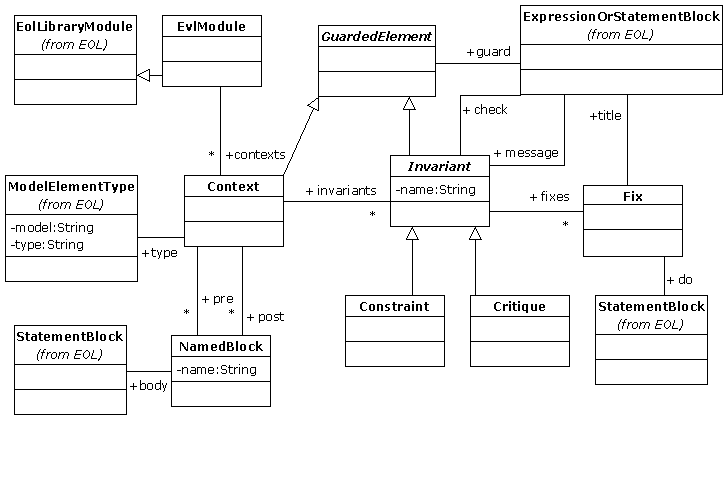
\includegraphics{images/EvlAbstractSyntax.png}
	\caption{Abstract Syntax of EVL}
	\label{fig:EvlAbstractSyntax}
\end{figure}
\end{landscape}

\paragraph{Context} A context specifies the kind of instances on which the contained invariants will be evaluated. Each context can optionally define a guard which limits its applicability to a narrower subset of instances of its specified type. Thus, if the guard fails for a specific instance of the type, none of its contained invariants are evaluated.

\paragraph{Invariant} As with OCL, each EVL invariant defines a \emph{name} and a body (\emph{check}). However, it can optionally also define a \emph{guard} (defined in its abstract \emph{GuardedElement} supertype) which further limits its applicability to a subset of the instances of the type defined by the embracing \emph{context}. To achieve the requirement for detailed user feedback (Section \ref{sec:Issue1}), each invariant can optionally define a \emph{message} as an \emph{ExpressionOrStatementBlock} that should return a String providing a description of the reason(s) for which the constraint has failed on a particular element. To support semi-automatically fixing of elements on which invariants have failed (Section \ref{sec:Issue5}), an invariant can optionally define a number of \emph{fixes}. Finally, as displayed in Figure \ref{fig:EvlAbstractSyntax}, \emph{Invariant} is an abstract class that is used as a super-class for the specific types \emph{Constraint} and \emph{Critique}. This is to address the issue of separation of errors and warnings/critiques (Section \ref{sec:Issue2}).

\paragraph{Guard} Guards are used to limit the applicability of invariants (Section \ref{sec:Issue4}). This can be achieved at two levels. At the \emph{Context} level it limits the applicability of all invariants of the context and at the \emph{Invariant} level it limits the applicability of a specific invariant.

\paragraph{Fix}
A fix defines a title using an \emph{ExpressionOrStatementBlock} instead of a static String to allow users to specify context-aware titles (e.g. \emph{Rename class customer to Customer} instead of a generic \emph{Convert first letter to upper-case}). Moreover, the \emph{do} part is a statement block where the fixing functionality can be defined using EOL. The developer is responsible for ensuring that the actions contained in the \emph{fix} actually repair the identified inconsistency.

\paragraph{Constraint}
\emph{Constraints} in EVL are used to capture critical errors that invalidate the model. As discussed above, \emph{Constraint} is a sub-class of \emph{Invariant} and therefore inherits all its features.

\paragraph{Critique}
Unlike \emph{Constraints}, \emph{Critiques} are used to capture non-critical situations that do not invalidate the model, but should nevertheless be addressed by the user to enhance the quality of the model. This separation addresses the issue raised in Section \ref{sec:Issue2}.

\paragraph{Pre and Post}
An EVL module can define a number of named \emph{pre} and a \emph{post} blocks that contain EOL statements which are executed before and after evaluating the invariants respectively. These should not be confused with the pre-/post-condition annotations available for EOL user-defined operations (Section~\ref{sec:prep-cond-user}).

\section{Concrete Syntax}

Listings \ref{lst:ContextConcreteSyntax}, \ref{lst:InvariantConcreteSyntax} and \ref{lst:FixConcreteSyntax} demonstrate the concrete sytnax of the \emph{context}, \emph{invariant} and \emph{fix} abstract syntax constructs discussed above.

\begin{lstlisting}[caption=Concrete Syntax of an EVL context, label=lst:ContextConcreteSyntax, language=EVL, escapechar=!]
context !\textit{name}! !\textbf{\{}!

	(guard (!\textbf{:}\textit{expression}!)|(!\textbf{\{}\textit{statementBlock}\textbf{\}}!))?
	
	(!\textit{invariant}!)*
	
!\textbf{\}}!
\end{lstlisting}

\begin{lstlisting}[caption=Concrete Syntax of an EVL invariant, label=lst:InvariantConcreteSyntax, language=EVL, escapechar=!]
(@lazy)?
(constraint|critique) !\textit{name}! !\textbf{\{}!
	
	(guard (!\textbf{:}\textit{expression}!)|(!\textbf{\{}\textit{statementBlock}\textbf{\}}!))?
	
	(check (!\textbf{:}\textit{expression}!)|(!\textbf{\{}\textit{statementBlock}\textbf{\}}!))?
	
	(message (!\textbf{:}\textit{expression}!)|(!\textbf{\{}\textit{statementBlock}\textbf{\}}!))?
	
	(!\textit{fix}!)*
	
!\textbf{\}}
\end{lstlisting}

\begin{lstlisting}[float=t, caption=Concrete Syntax of an EVL fix, label=lst:FixConcreteSyntax, language=EVL, escapechar=!]
fix !\textbf{\{}!
	(guard (!\textbf{:}\textit{expression}!)|(!\textbf{\{}\textit{statementBlock}\textbf{\}}!))?
	
	(title (!\textbf{:}\textit{expression}!)|(!\textbf{\{}\textit{statementBlock}\textbf{\}}!))?
	
	do !\textbf{\{}!
		!\textit{statementBlock}!
	!\textbf{\}}!
	
!\textbf{\}}!
\end{lstlisting}

\emph{Pre} and \emph{post} blocks have a simple syntax that, as presented in Listing \ref{lst:EvlPrePostConcreteSyntax}, consists of the identifier (\emph{pre} or \emph{post}), an optional name and the set of statements to be executed enclosed in curly braces.

\begin{lstlisting}[float=t, caption=Concrete Syntax of Pre and Post blocks, label=lst:EvlPrePostConcreteSyntax, language=EVL]
(pre|post) <name> {
	statement+
}
\end{lstlisting}

%\subsection{Concepts reused from EOL}

%As EVL has been built atop EOL, it reuses the following constructs from the base-language:

%\paragraph{ExpressionOrStatementBlock} There are cases where users needs to calculate a value (e.g. in the \emph{message} of an \emph{invariant}, in the \emph{guard} of a \emph{context} etc). When the value can be calculated declaratively, this is preferred. However, for cases in which calculating the value requires complex computations, users can use an EOL statement block and use a \emph{ReturnStatement} to return the calculated value to the caller.

%\paragraph{StatementBlock} A statement block is a sequence of EOL statements that can optionally include one or more \emph{ReturnStatements} to return a calculated value to its caller.

\section{Execution Semantics}
\label{sec:Design.EVL.ExecutionSemantics}

Having discussed the abstract and concrete syntaxes of EVL, this section provides an informal discussion of the execution semantics of the language. The execution of an EVL module is separated into four phases:

%The additional concepts EVL provides also affect its execution semantics. Currently, an EVL module can only be executed in batch-mode (all invariants against all instances). In the future we plan to investigate how the additional structures that EVL provides affect approaches to incremental consistency checking such as those presented in \cite{Cabot06,Egyed06}. In this section we outline the execution semantics of the language in batch-mode.

\paragraph{Phase 1} Before any invariant is evaluated, the \emph{pre} sections of the module are executed in the order in which they have been specified.

\paragraph {Phase 2} For each \emph{context}, the instances of the meta-class it defines are collected. For each instance, the \emph{guard} of the \emph{context} is evaluated. If the \emph{guard} is satisfied, then for each non-lazy invariant contained in the context the invariant's \emph{guard} is also evaluated. If the \emph{guard} of the invariant is satisfied, the \emph{body} of the invariant is evaluated. In case the \emph{body} evaluates to \emph{false}, the \emph{message} part of the rule is evaluated and the produced message is added along with the instance, the invariant and the available \emph{fixes} to the \emph{ValidationTrace}. 

The execution order of an EVL module follows a top-down depth-first scheme that respects the order in which the \emph{contexts} and \emph{invariants} appear in the module. However, the execution order can change in case one of the \emph{satisfies}, \emph{satisfiesOne}, \emph{satisfiesAll} built-in operations, discussed in detail in the sequel, are called.

\paragraph{Phase 3} In this phase, the validation trace is examined for unsatisfied constraints and the user is presented with the message each one has produced. The user can then select one or more of the available \emph{fixes} to be executed. Execution of \emph{fixes} is performed in a transactional manner using the respective facilities provided by the model connectivity framework, as discussed in Section \ref{sec:EMC.ModelTransactionSupport}. This is to prevent runtime errors raised during the execution of a \emph{fix} from compromising the validated model by leaving it in an inconsistent state.

\paragraph{Phase 4} When the user has performed all the necessary \emph{fixes} or chooses to end Phase 3 explicitly, the \emph{post} section of the module is executed. There, the user can perform tasks such as serializing the validation trace or producing a summary of the validation process results.

\subsection{Capturing Dependencies Between Invariants}

As discussed in Section \ref{sec:Issue3}, it is often the case that invariants conceptually depend on each other. To allow users capture such dependencies, EVL provides the \emph{satisfies(invariant : String) : Boolean}, \emph{satisfiesAll(invariants : Sequence(String)) : Boolean} and \emph{satisfiesOne(invariants : Sequence(String)) : Boolean} built-in operations. Using these operations, an invariant can specify in its \emph{guard} other invariants which need to be satisfied for it to be meaningful to evaluate.

When one of these operations is invoked, if the required \emph{invariants} (either lazy or non-lazy) have been evaluated for the instances on which the operation is invoked, the engine will return their cached results; otherwise it will evaluate them and return their results.

\section{Intra-Model Consistency Checking Example}
\label{sec:EvlIntraModelExample}
This section presents a case study comparing EVL and OCL in the context of a common scenario. The purpose of the case study is to present readers with the concrete syntax of the language and demonstrate the benefits delivered by the additional constructs it facilitates.

\subsection{Scenario: The Singleton Pattern}

The \emph{singleton} pattern is a widely used object oriented pattern. A \emph{singleton} is a class for which \emph{exactly one instance is allowed} \cite{Larman}. In UML, a singleton is typically represented as a class which is stereotyped with a \verb|<<singleton>>| stereotype and which also defines a static operation named \emph{getInstance()} that returns the unique instance. 

To ensure that all singletons have been modelled correctly in a UML model one needs to evaluate the following invariants on all classes that are stereotyped with the \verb|<<singleton>>| stereotype:

\begin{itemize}
	\item DefinesGetInstance : Each stereotyped class must define a getInstance() method
	\item GetInstanceIsStatic : The getInstance() method must be static
	\item GetInstanceReturnsSame : The return type of the getInstance() method must be the class itself 
\end{itemize}

Obviously, invariants \emph{GetInstanceIsStatic} and \emph{GetInstanceReturnsSame} depend on \emph{DefinesGetInstance} because if the singleton does not define a \emph{getInstance()} operation, checking for the operation's scope and return type is meaningless. Moreover, in case an invariant fails, there are corrective actions (fixes) that users may want to perform semi-automatically: e.g. for \emph{DefinesGetInstance}, such an action would be to add the missing \emph{getInstance()} operation, for \emph{GetInstanceIsStatic} to change it to static and for \emph{GetInstanceRetunrsSame} to set the return type to the class itself. In the following sections OCL and EVL are used to express the three constraints and then the two solutions are compared.

\subsection{Using OCL to Express the Invariants}

Listing \ref{lst:CaseStudyOcl} shows the aforementioned invariants implemented in OCL.

\begin{lstlisting}[caption=OCL Module for Validating Singletons, label=lst:CaseStudyOcl, language=OCL2]
package Foundation::Core
    
		context Class 

		def isSingleton :
			let isSingleton : Boolean =
			self.stereotype->exists(s|s.name = 'singleton')
        
		def getInstanceOperation  : 
			let getInstanceOperation : Operation =
			self.feature->select(f|f.oclIsTypeOf(Operation) 
			and f.name = 'getInstance')->first().oclAsType(Operation)

		inv DefinesGetInstanceOperation : 
			if isSingleton 
				then getInstanceOperation.isDefined
				else true
			endif
    	
		inv GetInstanceOperationIsStatic :
			if isSingleton then
				if getInstanceOperation.isDefined 
					then getInstanceOperation.ownerScope = #classifier 
					else false
				endif
			else 
				true
			endif
    	
		inv GetOperationReturnsSame :
			if isSingleton then
				if getInstanceOperation.isDefined then
					if getInstanceOperation.returnParameter.isDefined
						then getInstanceOperation.returnParameter.type = self 
						else false
					endif
				else
					false
				endif
			else 
				true
			endif
    	
    context Operation
        
		def returnParameter :
			let returnParameter : Parameter =
			self.parameter->select(p|p.kind = #return)->first()

endpackage

\end{lstlisting}

By examining the OCL solution it can be observed that all invariants first check that the class is a singleton (lines 15, 21 and 31) by using the \emph{isSingleton} derived property defined in line 5. If the isSingleton returns \emph{false}, the invariants return \emph{true} since returning false would cause them to fail for all non-singleton classes. This reveals an additional shortcoming of OCL: if a constraint returns \emph{true} it may mean two different things: either that the instance satisfies the constraint or that the constraint is not applicable to the instance at all. In our view, this overloading reduces understandability.

By further studying the solution of Listing \ref{lst:CaseStudyOcl} it can be noticed that dependency between constraints is captured artificially using nested \emph{if} expressions. For instance, both \emph{GetInstanceIsStatic} and \emph{GetInstanceRetunrsSame} contain an \emph{if} expression in lines 22 and 32 respectively, requiring that they recalculate the value of the \emph{getInstanceOperation} defined in line 9, where they actually recalculate the result of the \emph{DefinesGetInstanceOperation} invariant. As discussed in Section \ref{sec:Issue3}, this happens because OCL lacks constructs for capturing dependencies in a structured manner.

\subsection{Using EVL to Express the Invariants}

Listing \ref{lst:CaseStudy} provides a solution for this problem expressed in EVL.

\begin{lstlisting}[basicstyle=\ttfamily\footnotesize, flexiblecolumns=true, numbers=none, nolol=true, caption=EVL Module for Validating Singletons, label=lst:CaseStudy, numbers=left, language=EVL, tabsize=2]
context Singleton typeOf Class {
	
	guard : self.stereotype->exists(s|s.name = 'singleton')
	
	constraint DefinesGetInstance {
		check : self.getGetInstanceOperation()->isDefined()
		message : 'Singleton ' + self.name + 
			' must define a getInstance() operation'
		fix {
			title : 'Add a getInstance() operation to ' + self.name
			do {
				-- Create the getInstance operation
				var op : new Operation;
				op.name := 'getInstance';
				op.owner := self;
				op.ownerScope := ScopeKind#sk_classifier;
				
				-- Create the return parameter
				var returnParameter : new Parameter;
				returnParameter.type := self;
				op.parameter := Sequence{returnParameter};
				returnParameter.kind := ParameterDirectionKind#pdk_return;
			}
		}
	}
	
	constraint GetInstanceIsStatic {
		guard : self.satisfies('DefinesGetInstance')
		check : self.getGetInstanceOperation().ownerScope = 
		        ScopeKind#sk_classifier
		message : ' The getInstance() operation of singleton ' 
		          + self.name + ' must be static'
	
		fix {
			title : 'Change to static'
			do {
				self.getGetInstanceOperation.ownerScope 
				  := ScopeKind#sk_classifier;
			}
		}
	}
	
	constraint GetInstanceReturnsSame {
	
		guard : self.satisfies('DefinesGetInstance')
		check {
			var returnParameter : Parameter;
			returnParameter := self.getReturnParameter();
			return (returnParameter->isDefined() 
			        and returnParameter.type = self);
		}
		message : ' The getInstance() operation of singleton ' 
		          + self.name + ' must return ' + self.name
			
		fix {
			title : 'Change return type to ' + self.name
			do {
				var returnParameter : Parameter;
				returnParameter := self.getReturnParameter();
				
				-- If the operation does not have a return parameter
				-- create one
				if (not returnParameter.isDefined()){
					returnParameter := Parameter.newInstance();
					returnParameter.kind := ParameterDirectionKind#pdk_return;
					returnParameter.behavioralFeature := 
						self.getInstanceOperation();
				}
				-- Set the correct return type
				returnParameter.type := self;
			}
		}
	}
}

operation Class getGetInstanceOperation() : Operation {
	return self.feature->
		select(o:Operation|o.name = 'getInstance').first();
}

operation Operation getReturnParameter() : Parameter {
	return self.parameter->
		select(p:Parameter|p.kind = 
			ParameterDirectionKind#pdk_return).first();
}
\end{lstlisting}

The \emph{Singleton} context defines that the invariants it contains will be evaluated on instances of the UML \emph{Class} type. Moreover, its guard defines that they will be evaluated only on classes that are stereotyped with the \emph{singleton} stereotype. Therefore, unlike the OCL solution of Listing \ref{lst:CaseStudyOcl}, invariants contained in this context do not need to check individually that the instances on which they are evaluated are singletons.

Constraint \emph{DefinesGetInstance} defines no guard which means that it will be evaluated for all the instances of the context. In its \emph{check} part, the constraint examines if the class defines an operation named \emph{getInstance()} by invoking the \emph{getGetInstanceOperation()} operation. If this fails, it proposes a fix that adds the missing operation to the class.

Constraint \emph{GetInstanceIsStatic} defines a guard which states that for the constraint to be evaluated on an instance, the instance must first satisfy the \emph{DefinesGetInstance} constraint. If it doesn't, it is not evaluated at all. In its \emph{check} part it examines that the \emph{getInstance()} operation is static. Note that here the constraint needs not check that the \emph{getInstance()} operation is defined again since this is assumed by the \emph{DefinesGetInstance} constraint on which it depends. If the constraint fails for an instance, the fix part can be invoked to change the scope of the \emph{getInstance()} operation to static.

Constraint \emph{GetInstanceReturnsSame} checks that the return type of the \emph{getInstance()} operation is the singleton itself. Similarly to the \emph{GetInstanceIsStatic} constraint, it defines that to be evaluated the \emph{DefinesGetInstance} constraint must be satisfied. If it fails for a particular instance, the fix part can be invoked. In the fix part, if the operation defines a return parameter of incorrect type, its type is changed and if it does not define a return parameter at all, the parameter is created and added to the parameters of the operation.

By observing the two solutions the OCL solution resembles the concept of defensive programming, where conditions are embedded in supplier code, while the EVL one is closer to the design by contract \cite{Meyer97} approach where conditions are explicitly checked in guards.

This case study has demonstrated that the additional constructs provided by EVL can reduce repetition significantly and thus enable specification of more concise constraints. Moreover, in case a constraint is not satisfied for a particular instance, the user is provided with a meaningful context-aware message and with automated facilities (fixes) for repairing the inconsistency.

\section{Inter-Model Consistency Checking Example}
\label{sec:EvlInterModelExample}

\begin{figure}[b]
	\centering
		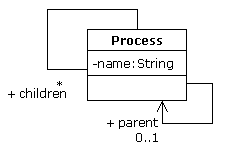
\includegraphics{images/Process.png}
	\caption{The ProcessLang Metamodel}
	\label{fig:Process}
\end{figure}

In the previous example, EVL was used to check the internal consistency of a single UML model. By contrast, this example demonstrates using EVL to detect and repair occurrences of incompleteness and contradiction between two different models. In this example the simplified \emph{ProcessLang} metamodel, which captures information about hierarchical processes, is used. To add performance information in a separate aspect \emph{ProcessPerformanceLang} metamodel is also defined. The metamodels are displayed in Figures \ref{fig:Process} and \ref{fig:ProcessPerformance} respectively.

\begin{figure}[b]
	\centering
		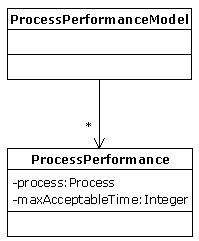
\includegraphics[width=0.2\textwidth]{images/ProcessPerformance.png}
	\caption{The ProcessPerformanceLang Metamodel}
	\label{fig:ProcessPerformance}
\end{figure}

There are two constraints that need to be defined and evaluated in this example: that each \emph{Process} in a process model (\emph{PM}) has a corresponding \emph{ProcessPerformance} in the process performance model (\emph{PPM}), and that the \emph{maxAcceptableTime} of a process does not exceed the sum of the \emph{maxAcceptableTimes} of its children. This is achieves with the \emph{PerformanceIsDefined} and the \emph{PerformanceIsValid} EVL constraints displayed in Listing \ref{lst:InterModelCaseStudy}.


\begin{lstlisting}[caption=Exemplar EVL module containing a cross-model constraint, label=lst:InterModelCaseStudy, language=EVL]
context PM!Process {	
	constraint PerformanceIsDefined { /*@\label{CaseStudy:PerformanceIsDefined}@*/
		
		check { /*@\label{CaseStudy:PerformanceIsDefined:Check}@*/
			var processPerformances = 
				PPM!ProcessPerformance.
				allInstances.select(pt|pt.process = self);
			
			return processPerformances.size() = 1;
		}
		
		message { /*@\label{CaseStudy:PerformanceIsDefined:Message}@*/
			var prefix : String;
			if (processPerformances.size() = 1) {
				prefix = "More than one performance info"; 
			}
			else {
				prefix = "No performance info";
			}
			return prefix + " found for process " 
				+ self.name;
		}
		
		fix { /*@\label{CaseStudy:PerformanceIsDefined:Fix}@*/
			title : "Set the performance of " + self.name
			
			do {
				for (p in processPerformances.clone()) {
					delete p;
				}
				var maxAcceptableTime : Integer;
				maxAcceptableTime = UserInput. /*@\label{CaseStudy:PerformanceIsDefined:Fix:Prompt}@*/
					promptInteger("maxAcceptableTime", 0); 
				var p : 
					new PPM!ProcessPerformance;
				p.maxAcceptableTime = maxAcceptableTime;
				p.process = self;
			}
		}
	}
	
	constraint PerformanceIsValid { /*@\label{CaseStudy:PerformanceIsValid}@*/
		
		guard : self.satisfies("PerformanceIsDefined") /*@\label{CaseStudy:PerformanceIsValid:Guard}@*/
			and self.children.forAll
				(c|c.satisfies("PerformanceIsDefined"))
		
		check { /*@\label{CaseStudy:PerformanceIsValid:Check}@*/
			var sum : Integer;
			sum = self.children. /*@\label{CaseStudy:PerformanceIsValid:Sum}@*/
				collect(c|c.getMaxAcceptableTime()) 
				.sum().asInteger(); 
			return self.getMaxAcceptableTime() >= sum;
		}
		
		message : "Process " + self.name + /*@\label{CaseStudy:PerformanceIsValid:Message}@*/
			" has a smaller maxAcceptableTime " 
			+ "than the sum of its children"
		
		fix { /*@\label{CaseStudy:PerformanceIsValid:Fix}@*/
			title : "Increase maxAcceptableTime to " + sum
			do {
				self.setMaxAcceptableTime(sum);
			}
		}
		
	}
	
}

operation PM!Process getMaxAcceptableTime() /*@\label{CaseStudy:getMaxAcceptableTime}@*/
	: Integer { 
	return PPM!ProcessPerformance.
		allInstances.selectOne(pt|pt.process=self)
			.maxAcceptableTime;
}

operation PM!Process setMaxAcceptableTime /*@\label{CaseStudy:setMaxAcceptableTime}@*/
	(time : Integer) { 
	PPM!ProcessPerformance.allInstances.
		selectOne(pt|pt.process=self).maxAcceptableTime =
		time;
}
\end{lstlisting}

In line \ref{CaseStudy:PerformanceIsDefined:Check}, the check part of the \emph{PerformanceIsDefined} constraint calculates the instances of \emph{ProcessPerformance} in the \emph{ProcessPerformanceModel} that have their \emph{process} reference set to the currently examined \emph{Process} (accessible via the \emph{self} built-in variable) and stores it in the \emph{processPerformances} variable. If exactly one \emph{ProcessPerformance} is defined for the \emph{Process}, the constraint is satisfied. Otherwise, the \emph{message} part of the constraint, in line \ref{CaseStudy:PerformanceIsDefined:Message}, is evaluated and an appropriate error message is displayed to the user. 

Note that the \emph{processPerformances} variable defined in the \emph{check} part is also used from within the \emph{message} part of the constraint. As discussed in \cite{EVL}, EVL provides this feature to reduce the need for duplicate calculations as our experience has shown that the message for a failed constraint often needs to utilize side-information collected in the \emph{check} part.

To repair the inconsistency, the user can invoke the \emph{fix} defined in line \ref{CaseStudy:PerformanceIsDefined:Fix} that will delete any existing \emph{ProcessPerformance} instances and create a new one with a user-defined \emph{maxAcceptableTime} obtained using the \emph{UserInput.promptInteger()} statement of line \ref{CaseStudy:PerformanceIsDefined:Fix:Prompt}.

Unlike the \emph{PerformanceIsDefined} constraint, the \emph{PerformanceIsValid} constraint, line \ref{CaseStudy:PerformanceIsValid}, defines a \emph{guard} part (line \ref{CaseStudy:PerformanceIsValid:Guard}). As discussed in \cite{EVL}, the guard part of a constraint is used to further limit the applicability of the constraint beyond the simple type check performed in the containing \emph{context}. In this rule, the validity of the \emph{maxAcceptableTime} of a \emph{Process} needs to be checked only if one has been defined in the \emph{ProcessPerformanceModel}. Therefore, the guard part of the constraint specifies that this constraint is only applicable to \emph{Processes} where, both they and they children, satisfy the \emph{PerformanceIsDefined} constraint.

The check part of the constraint retrieves the \emph{maxAcceptableTime} of the process and that of its children and compares them. As the \emph{Process} itself does not define performance information, retrieval of the value of the \emph{maxAcceptableTime} of the respective \emph{ProcessPerformance} object is implemented using the user-defined \emph{getMaxAcceptableTime()} operation that is defined in line \ref{CaseStudy:getMaxAcceptableTime}. In case the constraint is not satisfied, the user can invoke the \emph{fix} defined in line \ref{CaseStudy:PerformanceIsValid:Fix} to repair the inconsistency by setting the \emph{maxAcceptableTime} of the process to the \emph{sum} calculated in line \ref{CaseStudy:PerformanceIsValid:Sum}. As discussed earlier, the fix parts of EVL invariants do not in any way guarantee that they do fix the problem they target or that in their effort to fix one problem they do not create another problem; this is left to the user. For instance, in this particular example, changing the \emph{maxAcceptableTime} of a process through a \emph{fix} block may render its parent process invalid.

\begin{figure*}
	\centering
		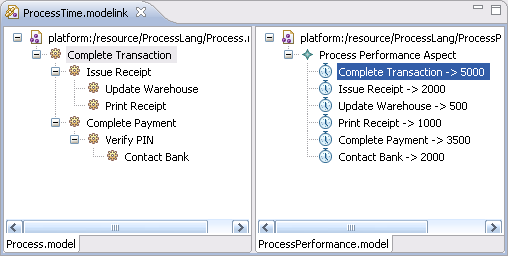
\includegraphics{images/ModeLink.png}
	\caption{Exemplar Process and ProcessPerformance models}
	\label{fig:ModeLink}
\end{figure*}

\begin{figure*}
	\centering
		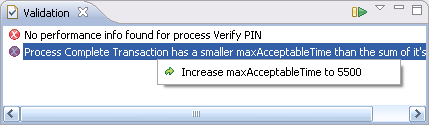
\includegraphics{images/Validation.png}
	\caption{Screenshot of the validation view reporting the identified inconsistencies}
	\label{fig:Validation}
\end{figure*}

To demonstrate the evaluation of these constraints two exemplar models that conform to the \emph{ProcessLang} and \emph{ProcessPerformanceLang} metamodels are used. A visual representation of the models is displayed in Figure \ref{fig:ModeLink}.

Evaluating the constraints in the context of those two models reveals two problems which are reported to the user via the view displayed in Figure \ref{fig:Validation}. Indeed by examining the two models of Figure \ref{fig:ModeLink}, it becomes apparent that there is no \emph{ProcessPerformance} linked to the \emph{Verify PIN} process and also that the \emph{maxAcceptableTime} of \emph{Complete Transaction} (5000) is less than the sum of the \emph{maxAcceptableTimes} of its children (2000 + 3500).

\section{Summary}

This section has provided a detailed discussion on the EVL model-validation language which conceptually (as opposed to technically) extends OCL. EVL provides a number of features such as support for detailed user feedback, constraint dependency management, semi-automatic transactional inconsistency resolution and (as it is based on EOL) access to multiple models of diverse metamodels and technologies.

%%% Local Variables:
%%% mode: latex
%%% TeX-master: "EpsilonBook"
%%% End:


\chapter{The Epsilon Transformation Language (ETL)}
\label{sec:ETL}

The aim of ETL \cite{ETL} is to contribute model-to-model transformation capabilities to Epsilon. More specifically, ETL can be used to transform an arbitrary number of input models into an arbitrary number of output models of different modelling languages and technologies at a high level of abstraction. 

\section{Style}

Three styles are generally recognized in model transformation languages: declarative, imperative and hybrid, each one demonstrating particular advantages and shortcomings. Declarative transformation languages are generally limited to scenarios where the source and target metamodels are similar to each other in terms of structure and thus, the transformation is a matter of a simple mapping. However they fail to address cases where significant processing and complex mappings are involved. On the other hand, purely imperative transformation languages are capable of addressing a wider range of transformation scenarios. Nevertheless, they operate at a low level of abstraction which means that users need to manually address issues such as tracing and resolving target elements from their source counterparts and orchestrating the transformation execution. To address those shortcomings, hybrid languages (such as ATL \cite{ATL} and QVT \cite{QVT}) provide both a declarative rule-based execution scheme as well as imperative features for handling complex transformation scenarios. 

Under this rationale, ETL has been designed as a hybrid language that implements a task-specific rule definition and execution scheme but also inherits the imperative features of EOL to handle complex transformations where this is deemed necessary.

\section{Source and Target Models}

The majority of model-to-model transformation languages assume that only two models participate in each transformation: the source model and the target model. Nevertheless, it is often essential to be able to access/update additional models during a transformation (such as trace or configuration models). Building on the facilities provided by EMC and EOL, ETL enables specification of transformations that can transform an arbitrary number of source models into an arbitrary number of target models.

Another common assumption is that the contents of the target models are insignificant and thus a transformation can safely overwrite its contents. As discussed in the sequel, ETL - like all Epsilon languages - enables the user to specify, for each involved model, whether its contents need to be preserved or not.

\section{Abstract Syntax}

As illustrated in Figure \ref{fig:EtlAbstractSyntax}, ETL transformations are organized in modules (\emph{EtlModule}). A module can contain a number of transformation rules (\emph{TransformationRule}). Each rule has a unique name (in the context of the module) and also specifies one \emph{source} and many \emph{target} parameters. A transformation rule can also \emph{extend} a number of other transformation rules and be declared as \emph{abstract}, \emph{primary} and/or \emph{lazy}\footnote{The concept of lazy rules was first introduced in ATL}. To limit its applicability to a subset of elements that conform to the type of the \emph{source} parameter, a rule can optionally define a guard which is either an EOL expression or a block of EOL statements. Finally, each rule defines a block of EOL statements (\emph{body}) where the logic for populating the property values of the target model elements is specified.

Besides transformation rules, an ETL module can also optionally contain a number of \emph{pre} and \emph{post} named blocks of EOL statements which, as discussed later, are executed before and after the transformation rules respectively. These should not be confused with the pre-/post-condition annotations available for EOL user-defined operations (Section~\ref{sec:prep-cond-user}).

\begin{landscape}
\begin{figure}
	\centering
		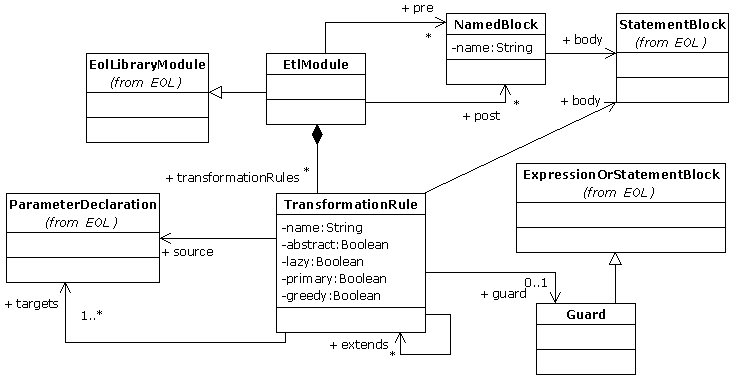
\includegraphics{images/EtlAbstractSyntax.png}
	\caption{ETL Abstract Syntax}
	\label{fig:EtlAbstractSyntax}
\end{figure}
\end{landscape}

\section{Concrete Syntax}

The concrete syntax of a transformation rule is displayed in Listing \ref{lst:TransformationRuleConcreteSyntax}. The optional \emph{abstract}, \emph{lazy} and \emph{primary} attributes of the rule are specified using respective annotations. The name of the rule follows the \emph{rule} keyword and the \emph{source} and \emph{target} parameters are defined after the \emph{transform} and \emph{to} keywords. Also, the rule can define an optional comma-separated list of rules it extends after the \emph{extends} keyword. Inside the curly braces (\{\}), the rule can optionally specify its \emph{guard} either as an EOL expression following a colon (:) (for simple guards) or as a block of statements in curly braces (for more complex guards). Finally, the \emph{body} of the rule is specified as a sequence of EOL statements.

\begin{lstlisting}[float=tbp, caption=Concrete Syntax of a TransformationRule, label=lst:TransformationRuleConcreteSyntax, language=ETL]
(@abstract)?
(@lazy)?
(@primary)?
rule <name> 
	transform <sourceParameterName>:<sourceParameterType>
	to (<rightParameterName>:<rightParameterType>
	(, <rightParameterName>:<rightParameterType>)*
	(extends (<ruleName>,)*<ruleName>)? {
	
	(guard (:expression)|({statement+}))?
	
	statement+
}
\end{lstlisting}

\emph{Pre} and \emph{post} blocks have a simple syntax that, as presented in Listing \ref{lst:EtlPrePostConcreteSyntax}, consists of the identifier (\emph{pre} or \emph{post}), an optional name and the set of statements to be executed enclosed in curly braces.

\begin{lstlisting}[float=tbp, caption=Concrete Syntax of Pre and Post blocks, label=lst:EtlPrePostConcreteSyntax, language=ETL]
(pre|post) <name> {
	statement+
}
\end{lstlisting}

\section{Execution Semantics}
\label{sec:ETL.ExecutionSemantics}

\subsection{Rule and Block Overriding}
Similarly to ECL, an ETL module can import a number of other ETL modules. In this case, the importing ETL module inherits all the rules and pre/post blocks specified in the modules it imports (recursively). If the module specifies a rule or a pre/post block with the same name, the local rule/block overrides the imported one respectively.

\subsection{Rule Execution Scheduling}

When an ETL module is executed, the \emph{pre} blocks of the module are executed first in the order in which they have been specified. 

Following that, each \emph{non-abstract} and \emph{non-lazy} rule is executed for all the elements on which it is applicable. To be applicable on a particular element, the element must have a kind-of relationship with the type defined in the rule's \emph{sourceParameter} and must also satisfy the \emph{guard} of the rule (and all the rules it extends). When a rule is executed on an applicable element, the target elements are initially created by instantiating the \emph{targetParameters} of the rules, and then their contents are populated using the EOL statements of the \emph{body} of the rule.

Finally, when all rules have been executed, the \emph{post} blocks of the module are executed in the order in which they have been declared.

\subsection{Source Elements Resolution}

Resolving target elements that have (or can be) transformed from source elements by other rules is a frequent task in the body of a transformation rule. To automate this task and reduce coupling between rules, ETL contributes the \emph{equivalents()} and \emph{equivalent()} built-in operations that automatically resolve source elements to their transformed counterparts in the target models. 

When the \emph{equivalents()} operation is applied on a single source element (as opposed to a collection of them), it inspects the established transformation trace (displayed in Figure \ref{fig:EtlRuntime}) and invokes the applicable rules (if necessary) to calculate the counterparts of the element in the target model. When applied to a collection it returns a \emph{Bag} containing \emph{Bags} that in turn contain the counterparts of the source elements contained in the collection. The \emph{equivalents()} operation can be also invoked with an arbitrary number of rule names as parameters to invoke and return only the equivalents created by specific rules. Unlike the main execution scheduling scheme discussed above, the \emph{equivalents()} operation invokes both \emph{lazy} and \emph{non-lazy} rules.

With regard to the ordering of the results of the \emph{equivalents()} operations, the returned elements appear in the respective order of the rules that have created them. An exception to this occurs when one of the rules is declared as \emph{primary}, in which case its results precede the results of all other rules.

ETL also provides the convenience \emph{equivalent()} operation which, when applied to a single element, returns only the first element of the respective result that would have been returned by the \emph{equivalents()} operation discussed above. Also, when applied to a collection the \emph{equivalent()} operation returns a flattened collection (as opposed to the result of \emph{equivalents()} which is a \emph{Bag} of \emph{Bags} in this case). As with the \emph{equivalents()} operation, the \emph{equivalent()} operation can also be invoked with or without parameters.

The semantics of the \emph{equivalent()} operation are further illustrated through a simple example. In this example, we need to transform a model that conforms to the Tree metamodel displayed in Figure \ref{fig:Tree} into a model that conforms to the Graph metamodel of Figure \ref{fig:Graph}. More specifically, we need to transform each \emph{Tree} element to a \emph{Node}, and an \emph{Edge} that connects it with the \emph{Node} that is equivalent to the tree's \emph{parent}. This is achieved using the rule of Listing \ref{lst:SimpleETLTransformationRule}. 

In lines \ref{lst:etl-simple-def-start}--\ref{lst:etl-simple-def-end}, the \emph{Tree2Node} rule specifies that it can transform elements of the \emph{Tree} type in the \emph{Tree} model into elements of the \emph{Node} type in the \emph{Graph} model. In line~\ref{lst:etl-simple-label} it specifies that the name of the created Node should be the same as the name of the source Tree. If the parent of the source \emph{Tree} is defined (line~\ref{lst:etl-simple-sourceisdef}), the rule creates a new \emph{Edge} (line~\ref{lst:etl-simple-newedge}) and sets its \emph{source} property to the created \emph{Node} (line~\ref{lst:etl-simple-source}) and its \emph{target} property to the \emph{equivalent} \emph{Node} of the source \emph{Tree}'s \emph{parent} (line~\ref{lst:etl-simple-equiv}).

\begin{figure}
	\centering
		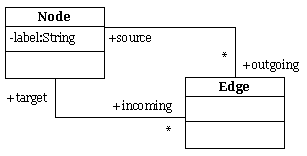
\includegraphics{images/Graph.png}
	\caption{A Simple Graph Metamodel}
	\label{fig:Graph}
\end{figure}

\begin{lstlisting}[float=tbp, caption=Exemplar ETL Rule demonstrating the \emph{equivalent()} operation, label=lst:SimpleETLTransformationRule, language=ETL, escapechar=\#]
rule Tree2Node#\label{lst:etl-simple-def-start}#
	transform t : Tree!Tree
	to n : Graph!Node {#\label{lst:etl-simple-def-end}#
	
	n.label = t.label;#\label{lst:etl-simple-label}#
	
	if (t.parent.isDefined()) {#\label{lst:etl-simple-sourceisdef}#
		var edge = new Graph!Edge;#\label{lst:etl-simple-newedge}#
		edge.source = n;#\label{lst:etl-simple-source}#
		edge.target = t.parent.equivalent();#\label{lst:etl-simple-equiv}#
	}
}
\end{lstlisting}

\begin{landscape}
\begin{figure}
	\centering
		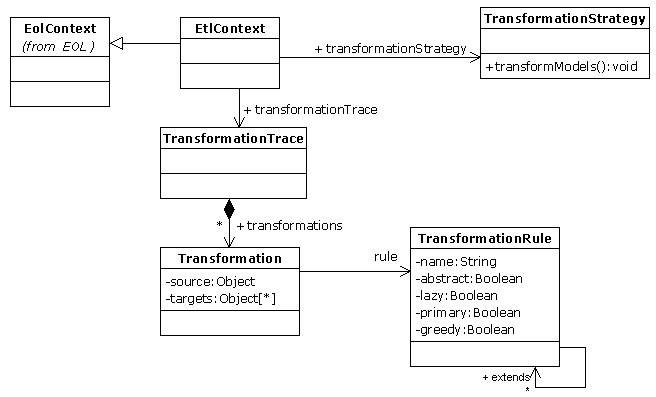
\includegraphics{images/EtlRuntime.png}
	\caption{ETL Runtime}
	\label{fig:EtlRuntime}
\end{figure}
\end{landscape}

\subsection{Overriding the semantics of the EOL SpecialAssignmentOperator}
\label{sec:Design.ETL.SpecialAssignmentOperator}

As discussed above, resolving the equivalent(s) or source model elements in the target model is a recurring task in model transformation. Furthermore, in most cases resolving the equivalent of a model element is immediately followed by assigning/adding the obtained target model elements to the value(s) of a property of another target model element. For example, in line 10 of Listing \ref{lst:SimpleETLTransformationRule} the \emph{equivalent} obtained is immediately assigned to the \emph{target} property of the generated \emph{Edge}. To make transformation specifications more readable, ETL overrides the semantics of the \emph{SpecialAssignmentStatement} (\emph{::=} in terms of concrete syntax), described in Section \ref{sec:Design.EOL.SpecialAssignmentStatement} to set its left-hand side, not to the element its right-hand side evaluates to, but to its \emph{equivalent} as calculated using the \emph{equivalent()} operation discussed above. Using this feature, line 10 of the \emph{Tree2Node} rule can be rewritten as shown in Listing \ref{lst:SpecialAssignmentETLTransformationRule}

\begin{lstlisting}[float=tbp, caption=Rewritten Line 10 of the \emph{Tree2Node} Rule Demonstrated in Listing \ref{lst:SimpleETLTransformationRule}, label=lst:SpecialAssignmentETLTransformationRule, language=ETL]
edge.target ::= t.parent;
\end{lstlisting}


\section{Interactive Transformations}
\label{sec:InteractiveModelTransformation}

Using the user interaction facilities of EOL discussed in Section \ref{sec:Design.EOL.UserInput}, an ETL transformation can become interactive by prompting the user for input during its execution. For example in Listing \ref{lst:InteractiveETLTransformationRule}, we modify the \emph{Tree2Node} rule originally presented in Listing \ref{lst:SimpleETLTransformationRule} by adding a \emph{guard} part that uses the user-input facilities of EOL (more specifically the \emph{UserInput.confirm(String,Boolean)} operation) to enable the user select manually at runtime which of the Tree elements need to be transformed to respective Node elements in the target model and which not. 

\begin{lstlisting}[float=tbp, caption=Exemplar Interactive ETL Transformation, label=lst:InteractiveETLTransformationRule, language=ETL]
rule Tree2Node
	transform t : Tree!Tree
	to n : Graph!Node {
	
	guard : UserInput.confirm
		("Transform tree " + t.label + "?", true)
	
	n.label = t.label;
	var target : Graph!Node ::= t.parent;
	if (target.isDefined()) {
		var edge = new Graph!Edge;
		edge.source = n;
		edge.target = target;
	}
}
\end{lstlisting}

\section{Summary}

This section has provided a detailed discussion on the Epsilon Transformation Language (ETL). ETL is capable of transforming an arbitrary number of source models into an arbitrary number of target models. ETL adopts a hybrid style and features declarative rule specification using advanced concepts such as \emph{guards}, \emph{abstract}, \emph{lazy} and \emph{primary} rules, and automatic resolution of target elements from their source counterparts. Also, as ETL is based on EOL reuses its imperative features to enable users to specify particularly complex, and even interactive, transformations.

\chapter{The Epsilon Wizard Language (EWL)}
\label{sec:EWL}

There are two types of model-to-model transformations: mapping and update transformations \cite{Czarnecki2003}. Mapping transformations typically transform a source model into a set of target models expressed in (potentially) different modelling languages by creating zero or more model elements in the target models for each model element of the source model. By contrast, update transformations perform in-place modifications in the source model itself. They can be further classified into two subcategories: transformations in the small and in the large. Update transformations in the large apply to sets of model elements calculated using well-defined rules in a batch manner. An example of this category of transformations is a transformation that automatically adds accessor and mutator operations for all attributes in a UML model. On the other hand, update transformations in the small are applied in a user-driven manner on model elements that have been explicitly selected by the user. An example of this kind of transformations is a transformation that renames a \emph{user-specified} UML class and all its incoming associations consistently.

In Epsilon, mapping transformations can be specified using ETL as discussed in Section \ref{sec:ETL}, and update transformations in the large can be implemented either using the model modification features of EOL or using an ETL transformation in which the source and target models are the same model. By contrast, update transformations in the small cannot be effectively addressed by any of the languages presented so far.

The following section discusses the importance of update transformations in the small and motivates the definition of a task-specific language (Epsilon Wizard Language (EWL)) that provides tailored and effective support for defining and executing update transformations on models of diverse metamodels.

\section{Motivation}
\label{sec:EwlMotivation}

Constructing and refactoring models is undoubtedly a mentally intensive process. However, during modelling, recurring patterns of model update activities typically appear. As an example, when renaming a class in a UML class diagram, the user also needs to manually update the names of association ends that link to the renamed class. Thus, when renaming a class from \emph{Chapter} to \emph{Section}, all associations ends that point to the class and are named \emph{chapter} or \emph{chapters} should be also renamed to \emph{section} and \emph{sections} respectively. As another example, when a modeller needs to refactor a UML class into a singleton \cite{Larman}, they need to go through a number of well-defined, but trivial, steps such as attaching a stereotype ($<<singleton>>$), defining a static \emph{instance} attribute and adding a static \emph{getInstance()} method that returns the unique instance of the singleton.

It is generally accepted that performing repetitive tasks manually is both counter-productive and error-prone \cite{CG.InAction}. On the other hand, failing to complete such tasks correctly and precisely compromises the consistency, and thus the quality, of the models. In Model Driven Engineering, this is particularly important since models are increasingly used to automatically produce (parts of) working systems. 

\subsection{Automating the Construction and Refactoring Process}

Contemporary modelling tools provide built-in transformations (\textit{wizards}) for automating common repetitive tasks. However, according to the architecture of the designed system and the specific problem domain, additional repetitive tasks typically appear, which cannot be addressed by the pre-conceived built-in wizards of a modelling tool. To address the automation problem in its general case, users must be able to easily define update transformations (wizards) that are tailored to their specific needs.

To an extent, this can be achieved via the extensible architecture that state-of-the-art modelling tools often provide and which enables users to add functionality to the tool via scripts or application code using the implementation language of the tool. Nevertheless, as discussed in \cite{EOL}, the majority of modelling tools provide an API through which they expose an edited model, which requires significant effort to learn and use. Also, since each API is proprietary, such scripts and extensions are not portable to other tools. Finally, API scripting languages and third-generation languages such as Java and C++ are not particularly suitable for model navigation and modification \cite{EOL}.

Furthermore, existing languages for mapping transformations, such as QVT, ATL and ETL, cannot be used as-is for this purpose, because these languages have been designed to operate in a batch manner without human involvement in the process. By contrast, as discussed above, the task of constructing and refactoring models is inherently user-driven.

\section{Update Transformations in the Small}
\label{sec:ModelTransformationInTheSmall}

Update transformations are actions that automatically create, update or delete model elements based on a selection of existing elements in the model and information obtained otherwise (e.g. through user input), in a user-driven fashion. In this section such actions are referred to as \textit{wizards} instead of \textit{rules} to reduce confusion between them and rules of mapping transformation languages. In the following sections the desirable characteristics of wizards are elaborated informally. 

\subsection{Structure of Wizards}

In its simplest form, a wizard only needs to define the actions it will perform when it is applied to a selection of model elements. The structure of such a wizard that transforms a UML class into a \textit{singleton} is shown using pseudo-code in Listing \ref{lst:Basic}.\\

\begin{lstlisting}[caption=The simplest form of a wizard for refactoring a class into a singleton, label=lst:Basic, language=EWL]
do :
	attach the singleton stereotype
	create the instance attribute
	create the getInstance method
\end{lstlisting}

Since not all wizards apply to all types of elements in the model, each wizard needs to specify the types of elements to which it applies. For example, the wizard of Listing \ref{lst:Basic}, which automatically transforms a class into a singleton, applies only when the selected model element is a class. The simplest approach to ensuring that the wizard will only be applied on classes is to enclose its body in an \emph{if} condition as shown in Listing \ref{lst:WithoutGuard}.

\begin{lstlisting}[caption=The wizard of Listing \ref{lst:Basic} enhanced with an $if$ condition, label=lst:WithoutGuard, language=EWL]
do : 
	if (selected element is a class) {
		attach the singleton stereotype
		create the instance attribute
		create the getInstance method
	}
\end{lstlisting}

A more modular approach is to separate this condition from the body of the wizard. This is shown in Listing \ref{lst:WithGuard} where the condition of the wizard is specified as a separate \emph{guard} stating that the wizard applies only to elements of type Class. The latter is preferable since it enables filtering out wizards that are not applicable to the current selection of elements by evaluating only their \emph{guard} parts and rejecting those that return \emph{false}. Thus, at any time, the user can be provided with only the wizards that are applicable to the current selection of elements. Filtering out irrelevant wizards reduces confusion and enhances usability, particularly as the list of specified wizards grows.

\begin{lstlisting}[caption=The wizard of Listing \ref{lst:WithoutGuard} with an explicit $guard$ instead of the $if$ condition, label=lst:WithGuard, language=EWL]
guard : selected element is a class
do : 
	attach the singleton stereotype
	create the instance attribute
	create the getInstance method
\end{lstlisting}

To enhance usability, a wizard also needs to define a short human-readable description of its functionality. To achieve this, another field named \emph{title} has been added. There are two options for defining the title of a wizard: the first is to use a static string and the second to use a dynamic expression. The latter is preferable since it enables definition of context-aware titles.

\begin{lstlisting}[caption=The wizard of Listing \ref{lst:WithGuard} enhanced with a $title$ part, label=lst:FinalForm, language=EWL]
guard : selected element is a class
title : Convert class <class-name> into a singleton
do : 
	attach the singleton stereotype
	create the instance attribute
	create the getInstance method
\end{lstlisting}

\subsection{Capabilities of Wizards}

The \emph{guard} and \emph{title} parts of a wizard need to be expressed using a language that provides model querying and navigation facilities. Moreover, the \emph{do} part also requires model modification capabilities to implement the transformation. To achieve complex transformations, it is essential that the user can provide additional information. For instance, to implement a wizard that addresses the class renaming scenario discussed in Section \ref{sec:EwlMotivation}, the information provided by the selected class does not suffice; the user must also provide the new name of the class. Therefore, EWL must also provide mechanisms for capturing user input.

\section{Abstract Syntax}

Since EWL is built atop Epsilon, its abstract and concrete syntax need only to define the concepts that are relevant to the task it addresses; they can reuse lower-level constructs from EOL. A graphical overview of the abstract syntax of the language is provided in Figure \ref{fig:EwlAbstractSyntax}. 

The basic concept of the EWL abstract syntax is a \emph{Wizard}. A wizard defines a \emph{name}, a \emph{guard} part, a \emph{title} part and a $do$ part. Wizards are organized in \emph{Modules}. The \emph{name} of a wizard acts as an identifier and must be unique in the context of a module. The \emph{guard} and \emph{title} parts of a wizard are of type \emph{ExpressionOrStatementBlock}, inherited from EOL. An \emph{ExpressionOrStatementBlock} is either a single EOL expression or a block of EOL statements that include one or more \emph{return} statements. This construct allows users to express simple declarative calculations as single expressions and complex calculations as blocks of imperative statements. The usefulness of this construct is further discussed in the examples presented in Section \ref{sec:EwlExamples}. Finally, the \emph{do} part of the wizard is a block of EOL statements that specify the effects of the wizard when applied to a compatible selection of model elements. 

\begin{figure}
	\centering
		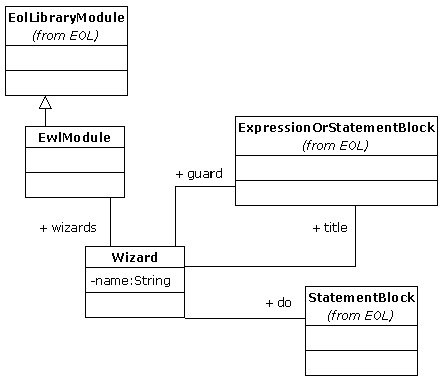
\includegraphics{images/EwlAbstractSyntax.png}
	\caption{EWL Abstract Syntax}
	\label{fig:EwlAbstractSyntax}
\end{figure}

\clearpage

\section{Concrete Syntax}

Listing \ref{lst:EwlConcreteSyntax} presents the concrete syntax of EWL wizards.

\begin{lstlisting}[caption=Concrete syntax of EWL wizards, label=lst:EwlConcreteSyntax, language=EWL, escapechar=!]
wizard !\textit{<name>}! {
	(guard (!\textbf{:}\textit{expression}!)|(!\textbf{\{}\textit{statementBlock}\textbf{\}}!))?
	(title (!\textbf{:}\textit{expression}!)|(!\textbf{\{}\textit{statementBlock}\textbf{\}}!))?
	do {
		statementBlock
	}
}
\end{lstlisting}

\section{Execution Semantics}
The process of executing EWL wizards is inherently user-driven and as such it depends on the environment in which they are used. In general, each time the selection of model elements changes (i.e. the user selects or deselects a model element in the modelling tool), the guards of all wizards are evaluated. If the guard of a wizard is satisfied, the \emph{title} part is also evaluated and the wizard is added to a list of \textit{applicable} wizards. Then, the user can select a wizard and execute its \emph{do} part to perform the intended transformation.

In EWL, variables defined and initialized in the \emph{guard} part of the wizard can be accessed both by the \emph{title} and the \emph{do} parts. In this way, results of calculations performed in the \emph{guard} part can be re-used, instead of re-calculated in the subsequent parts.  The practicality of this approach is discussed in more detail in the examples that follow. Also, the execution of the \emph{do} part of each wizard is performed in a transactional mode by exploiting the transaction capabilities of the underlying model connectivity framework, so that possible logical errors in the \emph{do} part of a wizard do not leave the edited model in an inconsistent state. 

\section{Examples}
\label{sec:EwlExamples}

This section presents three concrete examples of EWL wizards for refactoring UML 1.4 models. The aim of this section is not to provide complete implementations that address all the sub-cases of each scenario but to provide enhanced understanding of the concrete syntax, the features and the capabilities of EWL to the reader. Moreover, it should be stressed again that although the examples in this section are based on UML models, by building on Epsilon, EWL can be used to capture wizards for diverse modelling languages and technologies.

\subsubsection{Converting a Class into a Singleton}
\label{sec:ClassToSingleton}

The singleton pattern \cite{Larman} is applied when there is a class for which only one instance can exist at a time. In terms of UML, a singleton is a class stereotyped with the $<<singleton>>$ stereotype, and it defines a static attribute named \emph{instance} which holds the value of the unique instance. It also defines a static \emph{getInstance()} operation that returns that unique instance. Wizard \emph{ClassToSingleton}, presented in Listing \ref{lst:ClassToSingleton}, simplifies the process of converting a class into a singleton by adding the proper stereotype, attribute and operation to it automatically.

\begin{lstlisting}[float=tbp, 
	basicstyle=\ttfamily\footnotesize, 
	flexiblecolumns=true,
	numbers=none,
	nolol=true,
	caption=Implementation of the ClassToSingleton Wizard, 
	label=lst:ClassToSingleton,
	numbers=left,
	language=EWL,
	tabsize=2
]
wizard ClassToSingleton {
	
	// The wizard applies when a class is selected
	guard : self.isTypeOf(Class)
	
	title : "Convert " + self.name + " to a singleton"
	
	do {
		// Create the getInstance() operation 
		var gi : new Operation; 
		gi.owner = self; 
		gi.name = "getInstance"; 
		gi.visibility = VisibilityKind#vk_public; 
		gi.ownerScope = ScopeKind#sk_classifier; 
		
		// Create the return parameter of the operation 
		var ret : new Parameter; 
		ret.type = self; 
		ret.kind = ParameterDirectionKind#pdk_return; 
		gi.parameter = Sequence{ret}; 
		
		// Create the instance field 
		var ins : new Attribute; 
		ins.name = "instance"; 
		ins.type = self; 
		ins.visibility = VisibilityKind#vk_private; 
		ins.ownerScope = ScopeKind#sk_classifier; 
		ins.owner = self; 
		
		// Attach the <<singleton>> stereotype 
		self.attachStereotype("singleton");
	}
}

// Attaches a stereotype with the specified name
// to the Model Element on which it is invoked
operation ModelElement attachStereotype(name : String) {
		var stereotype : Stereotype;
		
		// Try to find an existing stereotype with this name
		stereotype = Stereotype.allInstances.selectOne(s|s.name = name);
		
		// If there is no existing stereotype
		// with that name, create one
		if (not stereotype.isDefined()){
			stereotype = Stereotype.createInstance();
			stereotype.name = name;
			stereotype.namespace = self.namespace;
		}
		
		// Attach the stereotype to the model element
		self.stereotype.add(stereotype);
}
\end{lstlisting}

The \emph{guard} part of the wizard specifies that it is only applicable when the selection is a single UML class. The \emph{title} part specifies a context-aware title that informs the user of the functionality of the wizard and the \emph{do} part implements the functionality by adding the \emph{getInstance} operation (lines 10-14), the \emph{instance} attribute (lines 23-28) and the $<<singleton>>$ stereotype (line 31). 

The stereotype is added via a call to the \emph{attachStereotype()} operation. Attaching a stereotype is a very common action when refactoring UML models, particularly where UML profiles are involved, and therefore to avoid duplication, this reusable operation that checks for an existing stereotype, creates it if it does not already exists, and attaches it to the model element on which it is invoked has been specified.

An extended version of this wizard could also check for existing association ends that link to the class and for which the upper-bound of their multiplicity is greater than one and either disallow the wizard from executing on such classes (in the $guard$ part) or update the upper-bound of their multiplicities to one (in the $do$ part). However, the aim of this section is not to implement complete wizards that address all sub-cases but to provide a better  understanding of the concrete syntax and the features of EWL. This principle also applies to the examples presented in the sequel.
\subsubsection{Renaming a Class}
\label{sec:RenameClass}

The most widely used convention for naming attributes and association ends of a given class is to use a lower-case version of the name of the class as the name of the attribute or the association end. For instance, the two ends of a one-to-many association that links classes \texttt{Book} and \texttt{Chapter} are most likely to be named \texttt{book} and \texttt{chapters} respectively. When renaming a class (e.g. from \texttt{Chapter} to \texttt{Section}) the user must then manually traverse the model to find all attributes and association ends of this type and update their names (i.e. from \texttt{chapter} or \texttt{bookChapter} to \texttt{section} and \texttt{bookSection} respectively). This can be a daunting process especially in the context of large models. Wizard \texttt{RenameClass} presented in Listing \ref{lst:RenameClass} automates this process.

\begin{lstlisting}[float=tbp, 
	basicstyle=\ttfamily\footnotesize, 
	flexiblecolumns=true, 
	numbers=none, 
	nolol=true, 
	caption=Implementation of the RenameClass Wizard,
	label=lst:RenameClass, 
	numbers=left, 
	language=EWL, 
	tabsize=2
]
wizard RenameClass {
	
	// The wizard applies when a Class is selected
	guard : self.isKindOf(Class)
	
	title : "Rename class " + self.name
	
	do {
		var newName : String;
		
		// Prompt the user for the new name of the class
		newName = UserInput.prompt("New name for class " + self.name);
		if (newName.isDefined()) {
			var affectedElements : Sequence;
			
			// Collect the AssociationEnds and Attributes
			// that are affected by the rename
			affectedElements.addAll(
				AssociationEnd.allInstances.select(ae|ae.participant=self));
			affectedElements.addAll(
				Attribute.allInstances.select(a|a.type = self));
			
			var oldNameToLower : String;
			oldNameToLower = self.name.firstToLowerCase();
			var newNameToLower : String;
			newNameToLower = newName.firstToLowerCase();
			
			// Update the names of the affected AssociationEnds
			// and Attributes
			for (ae in affectedElements) {
					ae.replaceInName(oldNameToLower, newNameToLower);
					ae.replaceInName(self.name, newName);
			}
			self.name = newName;
		}
	}
	
}

// Renames the ModelElement on which it is invoked
operation ModelElement replaceInName
	(oldString : String, newString : String) {
	
	if (oldString.isSubstringOf(self.name)) {
		// Calculate the new name
		var newName : String;
		newName = self.name.replace(oldString, newString);
		
		// Prompt the user for confirmation of the rename
		if (UserInput.confirm
			("Rename " + self.name + " to " + newName + "?")) {
			// Perform the rename
			self.name = newName;
		}
	}
}
\end{lstlisting}
%\vspace{-8pt}
As with the \texttt{ClassToSingleton} wizard, the \texttt{guard} part of \texttt{RenameClass} specifies that the wizard is applicable only when the selection is a simple class and the \emph{title} provides a context-aware description of the functionality of the wizard. 

As discussed in Section \ref{sec:ModelTransformationInTheSmall}, the information provided by the selected class itself does not suffice in the case of renaming since the new name of the class is not specified anywhere in the existing model. In EWL, and in all languages that build on EOL, user input can be obtained using the built-in \texttt{UserInput} facility. Thus, in line 12 the user is prompted for the new name of the class using the \texttt{UserInput.prompt()} operation. Then, all the association ends and attributes that refer to the class are collected in the \texttt{affectedElements} sequence (lines 14-21). Using the \texttt{replaceInName} operation (lines 31 and 32), the name of each one is examined for a substring of the upper-case or the lower-case version of the old name of the class. In case the check returns true, the user is prompted to confirm (line 48) that the feature needs to be renamed. This further highlights the importance of user input for implementing update transformations with fine-grained user control. 
\subsubsection{Moving Model Elements into a Different Package}
\label{sec:MoveToPackage}

A common refactoring when modelling in UML is to move model elements, particularly Classes, between different packages. When moving a pair of classes from one package to another, the associations that connect them must also be moved in the target package. To automate this process, Listing \ref{lst:MoveToPackage} presents the \texttt{MoveToPackage} wizard.

\begin{lstlisting}[float=tbp, 
	basicstyle=\ttfamily\footnotesize, 
	flexiblecolumns=true, 
	numbers=none, 
	nolol=true, 
	caption=Implementation of the MoveToPackage Wizard, 
	label=lst:MoveToPackage, 
	numbers=left, 
	language=EWL, 
	tabsize=2
]
wizard MoveToPackage {
	
	// The wizard applies when a Collection of
	// elements, including at least one Package
	// is selected
	guard { 
		var moveTo : Package;
		if (self.isKindOf(Collection)) {
			moveTo = self.select(e|e.isKindOf(Package)).last();
		}
		return moveTo.isDefined();
	}
	
	title : "Move " + (self.size()-1) + " elements to " + moveTo.name
	
	do {
		// Move the selected Model Elements to the
		// target package
		for (me in self.excluding(moveTo)) {
			me.namespace = moveTo;
		}
		
		// Move the Associations connecting any
		// selected Classes to the target package
		for (a in Association.allInstances) {
			if (a.connection.forAll(c|self.includes(c.participant))){
				a.namespace = moveTo;
			}
		}
	}
	
}
\end{lstlisting}

The wizard applies when more than one element is selected and at least one of the elements is a \emph{Package}. If more than one package is selected, the last one is considered as the target package to which the rest of the selected elements will be moved. This is specified in the \emph{guard} part of the wizard.

To reduce user confusion in identifying the package to which the elements will be moved, the name of the target package appears in the title of the wizard. This example shows the importance of the decision to express the title as a dynamically calculated expression (as opposed to a static string). It is worth noting that in the \emph{title} part of the wizard (line 14), the \emph{moveTo} variable declared in the \emph{guard} (line 7) is referenced. Through experimenting with a number of wizards, it has been noticed that in complex wizards repeated calculations need to be performed in the \emph{guard}, \emph{title} and \emph{do} parts of the wizard. To eliminate this duplication, the scope of variables defined in the \emph{guard} part has been extended so that they are also accessible from the \emph{title} and \emph{do} part of the wizard.


\section{Summary}

This section has presented the Epsilon Wizard Language (EWL), a language for specifying and executing update transformations in the small on models of diverse metamodels. EWL provides a textual concrete syntax tailored to the task and features such as dynamically calculated wizard titles, transactional execution of the \emph{do} parts of wizards and user interaction.

%!TEX root = ./EpsilonBook.tex

\chapter{The Epsilon Generation Language (EGL)}
\label{sec:EGL}
EGL provides a language tailored for model-to-text transformation (M2T). EGL can be used to transform models into various types of textual artefact, including executable code (e.g. Java), reports (e.g. in HTML), images (e.g. using DOT), formal specifications (e.g. Z notation), or even entire applications comprising code in multiple languages (e.g. HTML, Javascript and CSS).

EGL is a \emph{template-based} code generator (i.e. EGL programs resemble the text that they generate), and provides several features that simplify and support the generation of text from models, including: a sophisticated and language-independent merging engine (for preserving hand-written sections of generated text), an extensible template system (for generating text to a variety of sources, such as a file on disk, a database server, or even as a response issued by a web server), formatting algorithms (for producing generated text that is well-formatted and hence readable), and traceability mechanisms (for linking generated text with source models). 

% TODO: improve merge engine section: running example and describe how to use protected regions in the generated text
% TODO: improve traceability section

\section{Abstract Syntax}
Figure \ref{fig:abstractsyntax} depicts the abstract syntax of EGL's core functionality.

\begin{figure}[htbp]
  \begin{center}
    \leavevmode
    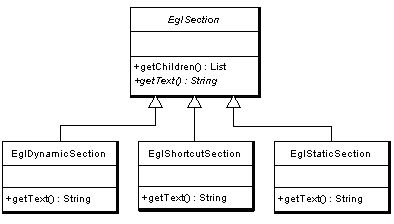
\includegraphics[scale=0.80]{images/EglAbstractSyntax.png}
  \end{center}
  \caption{The abstract syntax of EGL's core.}
  \label{fig:abstractsyntax}
\end{figure}

Conceptually, an EGL program comprises one or more \emph{sections}. The contents of static sections are emitted verbatim and appear directly in the generated text. The contents of dynamic sections are executed and are used used to control the text that is generated.

In its dynamic sections, EGL re-uses EOL's mechanisms for structuring program control flow, performing model inspection and navigation, and defining custom operations. In addition, EGL provides an EOL object, \verb|out|, which is used in dynamic sections to perform operations on the generated text, such as appending and removing strings; and specifying the type of text to be generated.

EGL also provides syntax for defining \textit{dynamic output} sections, which provide a convenient shorthand for outputting text from within dynamic sections. Similar syntax is often provided by
template-based code generators.

\section{Concrete Syntax}
\label{concretesyntax}

The concrete syntax of EGL closely resembles the style of other template-based code generation languages, such as PHP. The tag pair \emph{[\% \%]} is used to delimit a dynamic section. Any text not enclosed in such a tag pair is contained in a static section. Listing \ref{lst:basic} illustrates the use of dynamic and static sections to form a basic EGL template.

\begin{lstlisting}[float=tbp, caption=A basic EGL template., label=lst:basic, language=EGL]
[% for (i in Sequence{1..5}) { %]
i is [%=i%]
[% } %]
\end{lstlisting}

Executing the EGL template in Listing~\ref{lst:basic} would produce the generated text in Listing~\ref{lst:basic-generated}. The \emph{[\%=expr\%]} construct (line 2) is shorthand for \emph{[\%
  out.print(expr); \%]}, which appends \emph{expr} to the output generated by the transformation.

\begin{lstlisting}[float=tbp, caption=The text generated from the basic EGL template (Listing~\ref{lst:basic})., label=lst:basic-generated]
i is 1
i is 2
i is 3
i is 4
i is 5
\end{lstlisting}

Any EOL statement can be contained in the dynamic sections of an EGL template. For example, the EGL template depicted in Listing \ref{lst:oo} generates text from a model that conforms to a metamodel that describes an object-oriented system. % TODO include metamodel diagram

\begin{lstlisting}[float=tbp, caption=Generating the name of each Class contained in an input model., label=lst:oo, language=EGL]
[% for (c in Class.all) { %]
[%=c.name%]
[% } %]
\end{lstlisting}

\subsection{Comments and Markers}
Inside an EGL dynamic section, EOL's comment syntax can be used. Additionally, EGL adds syntax for comment blocks \texttt{[* this is a comment *]} and marker blocks \texttt{[*- this is a marker *]}. Marker blocks are highlighted by the EGL editor and EGL outline view in Eclipse.

\subsection{User-Defined Operations}

Like EOL, EGL permits users to define re-usable units of code via operations (Section~\ref{sec:Design.EOL.Operations}). EGL operations support the predefined annotations for regular EOL operations, such as optional pre-/post-conditions (Section~\ref{sec:prep-cond-user}) or
result caching (Section~\ref{sec:EolCaching}).

In EGL, user-defined operations are defined in dynamic sections, but may mix static and dynamic sections in their bodies. Consider, for example, the EGL code in Listing~\ref{lst:egl_operation}, which emits a declaration for a Java class (e.g. \texttt{public class Foo \{\}}). Lines 2-4 declare the operation. Note that the start and the end of the operation's declaration (on lines 2 and 4, respectively) are contained in dynamic sections. The body of the operation (line 3), however, mixes static and dynamic output sections. Finally, note that the operation is invoked from a dynamic section (line 1). It is worth noting that any loose (i.e. not contained in other operations) dynamic or static sections below the first operation of a template will be ignored at runtime.

\begin{lstlisting}[float=tbp, caption=Using an operation to specify the text generated for a declaration of a Java class., label=lst:egl_operation, language=EGL]
[% c.declaration(); %]
[% operation Class declaration() { %]
[%=self.visibility%] class [%=self.name%] {}
[% } %]
\end{lstlisting}

When a user-defined operation is invoked, any static or dynamic sections contained in the body of the operation are immediately appended to the generated text. Sometimes, however, it is desirable to manipulate the text produced by an operation before it is appended to the generated text. To this end, EGL defines the \texttt{@template} annotation which can applied to operations to indicate that any text generated by the operation must be returned from the operation and not appended to the generated text. For example, the EGL program in Listing~\ref{lst:egl_operation} could be rewritten using a \texttt{@template} annotation, as demonstrated in Listing~\ref{lst:egl_template_operation}.

\begin{lstlisting}[float=tbp, caption=Using a template operation to specify the text generated for a declaration of a Java class., label=lst:egl_template_operation, language=EGL]
[%=c.declaration()%]
[% @template
   operation Class declaration() { %]
[%=self.visibility%] class [%=self.name%] {}
[% } %]
\end{lstlisting}

There is a subtle difference between the way in which standard (i.e. unannotated) operations and \texttt{@template} operations are invoked. Compare the first line of Listings~\ref{lst:egl_operation} and~\ref{lst:egl_template_operation}. The former uses a dynamic section, because invoking the operation causes the evaluation of its body to be appended to the text generated by this program. By contrast, the latter uses a dynamic output section to append the result returned by the \texttt{@template} operation to the text generated by this program.

In general, \texttt{@template} operations afford more flexibility than standard operations. For example, line 1 of Listing~\ref{lst:egl_template_operation} could perform some manipulation of the text returned by the \texttt{declaration()} operation before the text is outputted. Therefore, \texttt{@template} operations provide a mechanism for re-using common pieces of a code generator, without sacrificing the flexibility to slightly alter text before it is emitted. Standard (unannotated) operations also permit re-use, but in a less flexible manner.

Finally, it is worth noting that user-defined operations in EGL do not have to generate text. For example, Listing~\ref{lst:egl_normal_operations} illustrates two operations defined in an EGL program that do not generate any text. The former is a query that returns a Boolean value, while the latter alters the model, and does not return a value.

\begin{lstlisting}[float=tbp, caption=Operations that do not generate any text., label=lst:egl_normal_operations, language=EGL]
[%
  operation Class isAnonymous() : Boolean {
		return self.name.isUndefined();
  }

  operation removeOneClass() {
		delete Class.all.random();
	}
%]
\end{lstlisting}

\section{The OutputBuffer}
As an EGL program is executed, text is appended to a data structure termed the \emph{OutputBuffer}. In every EGL program, the \emph{OutputBuffer} is accessible via the \texttt{out} built-in variable. The \emph{OutputBuffer} provides operations for appending to and removing from the buffer, and for merging generated text with existing text (see Section~\ref{sec:merging}).

For many EGL programs, interacting directly with the \emph{OutputBuffer} is unnecessary. The contents of static and dynamic output sections are sent directly to the \emph{OutputBuffer}, and no operation of the \emph{OutputBuffer} need be invoked directly. However, in cases when generated text must be sent to the \emph{OutputBuffer} from dynamic sections, or when generated text must be merged with existing text, the operations of \emph{OutputBuffer} (Table~\ref{tab:OutputBufferOperations}) are provided. Section~\ref{sec:merging} discusses merging generated and existing text, and presents several examples of invoking the operations of \emph{OutputBuffer}.

\begin{longtabu} {|p{6.5cm}|X|}
			
			\caption{Operations of type Template}
			\label{tab:OutputBufferOperations}\\
			
			\hline
							
			\textbf{Signature} & \textbf{Description} \\\hline
			
			chop(numberOfChars : Integer) & Removes the specified number of characters from the end of the buffer \\\hline
			
			print(object : Any) & Appends a string representation of the specified object to the buffer \\\hline
			
			println(object : Any) & Appends a string representation of the specified character and a new line to the buffer \\\hline
			
			println() & Appends a new line to the buffer \\\hline
			
			setContentType(contentType : String) & Updates the content type of this template. Subsequent calls to \texttt{pr\-es\-er\-ve} or \texttt{st\-a\-rtPr\-es\-er\-ve} that do not specify a style of comment will use the style of comment defined by the specified content type. See Section~\ref{sec:merging}. \\\hline
			
			preserve(id : String, enabled : Boolean, contents : String) & Appends a protected region to the buffer with the given identifier, enabled state and contents. Uses the current content type to determine how to format the start and end markers. See Section~\ref{sec:merging}. \\\hline
			
			preserve(startComment : String, endComment : String, id : String, enabled : Boolean, contents : String) & Appends a protected region to the buffer with the given identifier, enabled state and contents. Uses the first two parameters as start and end markers. See Section~\ref{sec:merging}. \\\hline
			
			startPreserve(id : String, enabled : Boolean) & Begins a protected region by appending the start marker for a protected region to the buffer with the given identifier and enabled state. Uses the current content type to determine how to format the start and end markers. See Section~\ref{sec:merging}. \\\hline
			
			startPreserve(startComment : String, endComment : String, id : String, enabled : Boolean) & Begins a protected region by appending the start marker to the buffer with the given identifier and enabled state. Uses the first two parameters as start and end markers. See Section~\ref{sec:merging}. \\\hline
			
			stopPreserve() & Ends the current protected region by appending the end marker to the buffer. This operation should be invoked only if there a protected region is currently open (i.e. has been started by invoking \texttt{st\-a\-rtPr\-es\-er\-ve} but not yet stopped by invoking \texttt{st\-opPr\-es\-er\-ve}). See Section~\ref{sec:merging}. \\\hline
\end{longtabu}

\section{Co-ordination}
\label{Co-ordination}
In the large, M2T transformations are used to generate text to various destinations. For example, code generators often produce files on disk, and web applications often generate text as part of the response for a resource on the web server. Text might be generated to a network socket during interprocess communication, or as a query that runs on a database. Furthermore, (parts of) a single M2T transformation might be re-used in different contexts. A M2T transformation that generates files on disk today might be re-purposed to generate the response from a web server tomorrow.  

Given these concerns, EGL provides a co-ordination engine that provides mechanisms for modularising M2T transformations, and for controlling the destinations to which text is generated. The EGL co-ordination engine fulfils three requirements:

\begin{enumerate}
	\item \textbf{Reusability}: the co-ordination engine allows EGL programs to be decomposed into one or more templates, which can be shared between EGL programs.

	\item \textbf{Variety of destination}: the co-ordination engine provides an extensible set of template types that can generate text to a variety of destinations. Section~\ref{sec:egl_template_type} describes the default template type, which is tailored to generate text to files on disk, while Section~\ref{sec:custom_co-ordination} discusses the way in  which users can define their own template types for generating text to other types of destination.
	
	\item \textbf{Separation of concerns}: the co-ordination engine ensures that the logic for controlling the text that is generated (i.e. the content) and the logic for controlling the way in which text is emitted (i.e. the destination) are kept separate.
\end{enumerate}

\subsection{The Template type}
\label{sec:egl_template_type}
Central to the co-ordination engine is the \emph{Template} type, which EGL provides in addition to the default EOL types (Section~\ref{sec:eol_types}). Via the \emph{Template} type, EGL fulfils the three requirements identified above. Firstly, a \emph{Template} can invoke other \emph{Templates}, and hence can be shared and re-used between EGL programs. Secondly, the \emph{Template} type has been implemented in an extensible manner: users can define their own types of \emph{Template} that generate text to any destination (e.g. a database or a network socket), as described in Section~\ref{sec:custom_co-ordination}. Finally, the \emph{Template} type provides a set of operations that are used to control the destination of generated text. Users typically define a ``driver'' template that does not generate text, but rather controls the destination of text that is generated by other templates. 

For example, consider the EGL program in Listing~\ref{lst:co-ordination}. This template generates no text (as it contains only a single dynamic section), but is used instead to control the destination of text generated by another template. Line 1 defines a variable, \texttt{t}, of type \emph{Template}. Note that, unlike the EOL types, instances of \emph{Template} are not created with the \texttt{new} keyword. Instead, the \emph{TemplateFactory} built-in object (Section~\ref{sec:template_factory}) is used to load templates from, for example, a file system path. On line 3, the \emph{generate} operation of the \emph{Template} type invokes the EGL template stored in the file ``ClassNames.egl'' and emits the generated text to ``Output.txt''.

\begin{lstlisting}[float=tbp, caption=Storing the name of each Class to disk., label=lst:co-ordination, language=EGL]
[%
  var t : Template = TemplateFactory.load("ClassNames.egl");
  t.generate("Output.txt");
%]
\end{lstlisting}

In addition to \texttt{generate}, the Template type defines further operations for controlling the context and invocation of EGL templates. Table~\ref{tab:TemplateOperations} lists all of the operations defined on \emph{Template}, and a further example of their use is given in Section~\ref{sec:example_of_co-ordination}.

\begin{longtabu} {|p{5.5cm}|X|}
			
			\caption{Operations of type Template}
			\label{tab:TemplateOperations}\\
			
			\hline
							
			\textbf{Signature} & \textbf{Description} \\\hline
			
			populate(name : String, value : Any) & Makes a variable with the specified name and value available during the execution of the template. \\\hline
			
			process() : String & Executes the template and returns the text that is generated.  \\\hline
			
			generate(destination : String) & Executes the template and stores the text to the specified destination. The format of the destination parameter is dictated by the type of template. For example, the default template type (which can generate files on disk) expects a file system path as the destination parameter. Returns a \class{java.io.File} object representing the generated file.\\\hline
			
			setFormatter(formatter : Formatter) & Changes the formatter for this template to the specified formatter. Subsequent calls to generate or process will produce text that is formatted with the specified formatter. See Section~\ref{sec:formatters}. \\\hline
			
			setFormatters(formatters : Sequence(Formatter)) & Changes the formatter for this template to the specified sequence of formatters. Subsequent calls to generate or process will produce text that is formatted with each of the specified formatters in turn. See Section~\ref{sec:formatters}. \\\hline
\end{longtabu}


\subsection{The TemplateFactory object}
As discussed above, instances of \emph{Template} are not created with the \texttt{new} keyword. Instead, EGL provides a built-in object, the \emph{TemplateFactory}, for this purpose. Users can customise the type of the \emph{TemplateFactory} object to gain more control over the way in which text is generated (Section~\ref{sec:custom_co-ordination}).

By default, EGL provides a \emph{TemplateFactory} that exposes operations for loading templates (by loading files from disk), preparing templates (by parsing a string containing EGL code), and for controlling the file system locations from which templates are loaded and to which text is generated. Table~\ref{tab:TemplateFactoryOperations} lists the operations provided by the built-in \emph{TemplateFactory} object. 

\label{sec:template_factory}
\begin{longtabu} {|p{5.5cm}|X|}
			
			\caption{Operations of the TemplateFactory object}
			\label{tab:TemplateFactoryOperations}\\
			
			\hline
							
			\textbf{Signature} & \textbf{Description} \\\hline
			
			load(path : String) : Template & Returns an instance of \emph{Template} that can be used to execute the EGL template stored at the specified path.  \\\hline
			
			prepare(code : String) : Template & Returns an instance of \emph{Template} that can be used to execute the specified EGL code.  \\\hline
			
			setOutputRoot(path : String) & Changes the default path that is used to resolve relative paths when generating files to disk. Subsequent calls to load and prepare will create templates that use the new path. \\\hline
			
			setTemplateRoot(path : String) & Changes the default path that is used to resolve relative paths when loading templates with the load operation. Subsequent calls to load will use the new path. \\\hline
			
			setDefaultFormatter(formatter : Formatter) & Changes the formatter for this template factory to the specified formatter. Templates that are constructed after this
operation has been invoked will produce text that is, by default, formatted with the specified formatter. See Section~\ref{sec:formatters}. \\\hline
			
			setDefaultFormatters(fo\-rm\-at\-te\-rs : Sequence(Formatter)) & Changes the formatter for this template to the specified sequence of formatters. Templates that are constructed after this operation has been invoked will produce text that is, by default, formatted with each of the specified formatters in turn. See Section~\ref{sec:formatters}.  \\\hline
\end{longtabu}

\subsection{An Example of Co-ordination with EGL}
\label{sec:example_of_co-ordination}
The operations provided by the \emph{TemplateFactory} object and \emph{Template} type are demonstrated by the EGL program in Listing~\ref{lst:co-ordination_complete}. Lines 2-3 use operations on \emph{TemplateFactory} to change the paths from which templates will be loaded (line 2) and to which generated files will be created (line 3). Line 5 demonstrates the use of the \texttt{prepare} operation for creating a template from EGL code. When the \texttt{interface} template is invoked, the EGL code passed to the \texttt{prepare} operation will be executed. Finally, line 9 (and line 12) illustrates the way in which the \texttt{populate} operation can be used to pass a value to a template before invoking it. Specifically, the interface and implementation templates can use a variable called \emph{root}, which is populated by the driver template before invoking them.

\begin{lstlisting}[float=tbp, caption=Using the various operations provided by the Template type and TemplateFactory object., label=lst:co-ordination_complete, language=EGL]
[%
  TemplateFactory.setTemplateRoot("/usr/franz/templates");
	TemplateFactory.setOutputRoot("/tmp/output");

  var interface      : Template =
    TemplateFactory.prepare("public interface [%=root.name] {}");
	
	var implementation : Template = 
	  TemplateFactory.load("Class2Impl.egl");

	for (c in Class.all) {
	  interface.populate("root", c);	
  	interface.generate("I" + c.name + ".java");
		
		implementation.populate("root", c);
		implementation.generate(c.name + ".java");
	}
%]
\end{lstlisting}

\subsection{Customising the Co-ordination Engine}
\label{sec:custom_co-ordination}
EGL provides mechanisms for customising the co-ordination engine. Specifically, users can define and use their own \emph{TemplateFactory}. In many cases, users need not customise the co-ordination engine, and can write transformations using the built-in \emph{Template} type and \emph{TemplateFactory} object. If, 
however, you need more control over the co-ordination process, the discussion in this section might be helpful. Specifically, a custom \emph{TemplateFactory} is typically used to achieve one or more of the following goals:


\begin{enumerate}
	\item Provide additional mechanisms for constructing \emph{Templates}. 
	      \textbf{Example:} facilitate the loading of templates from a database.
	\item Enrich / change the behaviour of the built-in \emph{Template} type.
	      \textbf{Example:} change the way in which generated text is sent to its destination.
	\item Observe or instrument the transformation process by, for instance, logging calls to
	      the operations provided by the \emph{Template} type of the \emph{TemplateFactory}
	      object.
	      \textbf{Example:} audit or trace the transformation process.
\end{enumerate}

Customisation is achieved in two stages: implementing the custom \emph{TemplateFactory} 
(and potentially a custom \emph{Template}) in Java, and using the custom 
\emph{TemplateFactory}. 

\subsubsection{Implementing a custom TemplateFactory}
A custom \emph{TemplateFactory} is a subclass of \texttt{EglTemplateFactory}. Typically, a custom \emph{TemplateFactory} is implemented by overriding one of the methods of \texttt{EglTemplateFactory}. For example, the \texttt{createTemplate} method is overriden to specify that a custom type of \emph{Template} should be created by the \emph{TemplateFactory}. Likewise, the \texttt{load} and \texttt{prepare} methods can be overriden to change the location from which \emph{Template}s are constructed.

A custom \emph{Template} is a subclass of \texttt{EglTemplate} or, most often, a subclass of \texttt{EglPersistentTemplate}. Again, customisation is typically achieved by overriding methods in the superclass, or by adding new methods. For example, to perform auditing activities whenever a template is used to generate text, the \texttt{doGenerate} method of \texttt{EglPersistentTemplate} is overriden.


\begin{lstlisting}[float=tbp, caption=A simple customisation of the co-ordination engine to count the number of calls to \texttt{generate()}., label=lst:custom_co-ordination_example, language=Java]
import org.eclipse.epsilon.egl.EglFileGeneratingTemplateFactory;
import org.eclipse.epsilon.egl.EglTemplate;
import org.eclipse.epsilon.egl.EglPersistentTemplate;
import org.eclipse.epsilon.egl.exceptions.EglRuntimeException;
import org.eclipse.epsilon.egl.execute.context.IEglContext;
import org.eclipse.epsilon.egl.spec.EglTemplateSpecification;

public class CountingTemplateFactory 
extends EglFileGeneratingTemplateFactory {

	@Override
	protected EglTemplate createTemplate(EglTemplateSpecification spec) 
	throws Exception {
		return new CountingTemplate(spec,
		                            context,
		                            getOutputRootOrRoot(),
		                            outputRootPath);
	}	

  public class CountingTemplate 
  extends EglPersistentTemplate {

		public static int numberOfCallsToGenerate = 0;

		public CountingTemplate(EglTemplateSpecification spec,
		                        IEglContext context,
		                        URI outputRoot,
		                        String outputRootPath)
		throws Exception {
			super(spec, context, outputRoot, outputRootPath);
		}



		@Override
		protected void doGenerate(File file,
			                        String targetName,
			                        boolean overwrite,
			                        boolean protectRegions) 
		throws EglRuntimeException {
			numberOfCallsToGenerate++;
		}
	}
}
\end{lstlisting}

\subsubsection{Using a custom TemplateFactory}
When invoking an EGL program, the user may select a custom \emph{TemplateFactory}. For example, the EGL development tools provide an Eclipse launch configuration that provides a tab named ``Generated Text.'' On this tab, users can select a \emph{TemplateFactory} (under the group called ``Type of Template Factory''). Note that a \emph{TemplateFactory} only appears on the launch configuration tab if it has been registered with EGL via an Eclipse extension. Similarly, the workflow language provided by Epsilon (Chapter~\ref{chp:Workflow}) allows the specification of custom types of \emph{TemplateFactory} via the \texttt{te\-m\-pl\-a\-teFa\-ct\-o\-ryTy\-pe} parameter.


\subsection{Summary}
The co-ordination engine provided by EGL facilitates the construction of modular and re-usable M2T transformations and can be used to generate text to various types of destination. Furthermore, the logic for specifying the contents of generated text is kept separate from the logic for specifying the destination of generated text.

\section{Merge Engine}
\label{sec:merging}
EGL provides language constructs that allow M2T transformations to designate regions of generated text as \textit{protected}. Whenever an EGL program attempts to generate text, any protected regions that are encountered in the specified destination are preserved.

Within an EGL program, protected regions are specified with the \emph{preserve(String, String,   String, Boolean, String)} method on the \verb|out| keyword. The first two parameters define the comment delimiters of the target language. The other parameters provide the name, enable-state and content of the protected region, as illustrated in Listing \ref{lst:preserve}. 

\begin{lstlisting}[float=tbp, caption=Protected region declaration using the preserve method., label=lst:preserve, language=EGL]
[%=out.preserve("/*", "*/", "anId", true,
                "System.out.println(foo);")
%]
\end{lstlisting}

A protected region declaration may have many lines, and use many EGL variables in the contents definition.  To enhance readability, EGL provides two additional methods on the \verb|out| keyword: \emph{startPreserve(String, String, String, Boolean)} and \verb|stopPreserve|.  Listing \ref{lst:startpreserve} uses these to generate a protected region equivalent to that in Listing \ref{lst:preserve}.

\begin{lstlisting}[float=tbp, caption=Protected region declaration., label=lst:startpreserve, language=EGL]
[%=out.startPreserve("/*", "*/", "anId", true)%]
System.out.println(foo);
[%=out.stopPreserve()%]
\end{lstlisting}

Because an EGL template may contain many protected regions, EGL also provides a separate method to set the target language generated by the current template, \emph{setContentType(String)}. By default, EGL recognises Java, HTML, Perl and EGL as valid content types. An alternative configuration file can be used to specify further content types. Following a call to \verb|setContentType|, the first two arguments to the \verb|preserve| and \verb|startPreserve| methods can be omitted, as shown in Listing \ref{lst:contenttype}.

\begin{lstlisting}[float=tbp, caption=Setting the content type., label=lst:contenttype, language=EGL]
[% out.setContentType("Java"); %]
[%=out.preserve("anId", true, "System.out.println(foo);")%]
\end{lstlisting}

Because some languages define more than one style of comment delimiter, EGL allows mixed use of  the styles for \verb|preserve| and \verb|startPreserve| methods.

Once a content type has been specified, a protected region may also be declared entirely from a static section, using the syntax in Listing \ref{lst:manualpr}.

\begin{lstlisting}[float=tbp, caption=Declaring a protected region from within a static section., label=lst:manualpr, language=EGL]
[% out.setContentType("Java"); %]
// protected region anId [on|off] begin
System.out.println(foo);
// protected region anId end
\end{lstlisting}

When a template that defines one or more protected regions is processed by the EGL execution engine, the target output destinations are examined and existing contents of any protected regions are preserved. If either the output generated by from the template or the existing contents of the target output destination contains protected regions, a merging process is invoked. Table \ref{tab:merging} shows the default behaviour of EGL's merge engine.

\begin{table}[htbp]
  \begin{center}
  \begin{tabular}{|l|l|l|}
  \hline
  \multicolumn{2}{|l|}{\textbf{Protected Region Status}} & \multirow{2}{*}{\textbf{Contents taken from}} \\
  \textbf{Generated} & \textbf{Existing} & \\
  \hline
  On & On     & Existing  \\
  On & Off    & Generated \\
  On & Absent & Generated \\
  \hline
  Off & On     & Existing  \\
  Off & Off    & Generated \\
  Off & Absent & Generated \\
  \hline
  Absent & On  & Neither (causes a warning) \\
  Absent & Off & Neither (causes a warning) \\
  \hline
  \end{tabular}
  \end{center}
\caption{EGL's default merging behaviour.}
\label{tab:merging}
\end{table}

\section{Formatters}
\label{sec:formatters}
Often the text generated by a model-to-text transformation is not formatted in a desirable  manner. Text generated with a model-to-text transformation might contain extra whitespace or inconsistent indentation. This is because controlling the formatting of generated text in a model-to-text transformation language can be challenging.

In a template-based model-to-text language, such as EGL, it can be difficult to know how best to format a transformation. On the one hand, the transformation must be readable and understandable, and on the other hand, the generated text must typically also be readable and understandable. 

Conscientious developers apply various \emph{conventions} to produce readable code. EGL encourages template developers to prioritise the readability of templates over the readability of generated text when 
writing EGL templates. For formatting generated text, EGL provides an extensible set of \textit{formatters} that can be invoked during a model-to-text transformation.

\subsection{Using a Formatter}
EGL provides several built-in formatters. Users can implement additional formatters (Section~\ref{sec:custom_formatter}). To use a formatter, invoke the \texttt{setFo\-rm\-at\-t\-er} or \texttt{setFo\-rm\-at\-te\-rs} operation on an instance of the \emph{Template} type. A formatter is a
Java class that implements EGL's Formatter interface. From within an EGL program, formatters can be created using a Native (i.e. Java) type. Listing~\ref{lst:programmatic_formatter} demonstrates the use of a built-in formatter (XmlFormatter).

\begin{lstlisting}[float=tbp, caption=Using a formatter from within an EGL program., label=lst:programmatic_formatter, language=EGL]
[%
	var f = new Native("org.eclipse.epsilon.egl.formatter.language.XmlFormatter");
	var t = TemplateFactory.load("generate_some_xml.egl");
	t.setFormatter(f);
	t.generate("formatted.xml");
%]
\end{lstlisting}

To facilitate the re-use of a formatter with many templates, the \emph{TemplateFactory} object provides the \texttt{setDe\-fa\-u\-ltFo\-rm\-at\-ter} and \texttt{setDe\-fa\-u\-ltFo\-rm\-at\-ters} operations. Templates that are loaded or prepared after a call to \texttt{setDe\-fa\-u\-ltFo\-rm\-at\-ter} or \texttt{setDe\-fa\-u\-ltFo\-rm\-at\-ters} will, by default, use the formatter(s) specified for the \emph{TemplateFactory}. Note that setting the formatter on a template overwrite any formatter that may have been set on that template by the \emph{TemplateFactory}.

The default formatters for an EGL program can also be set when invoking the program. For example, the EGL development tools provide an Eclipse launch configuration that provides a tab named ``Generated Text.'' On this tab, users can configure one or more formatters which will be used as the default formatters for this EGL program. Note that custom formatters only appear on the launch configuration tab if they have been registered with EGL via an Eclipse extension. Similarly, the workflow language provided by Epsilon (Chapter~\ref{chp:Workflow}) provides a \texttt{for\-ma\-tt\-er} nested element that can be used to specify one or more default formatters.

\subsection{Implementing a Custom Formatter}
\label{sec:custom_formatter}
Providing a user-defined formatter involves implementing the \texttt{Fo\-rm\-at\-ter} interface (in \texttt{org.eclipse.epsilon.egl.formatter}). For example, Listing~\ref{lst:custom_formatter} demonstrates a simple formatter that transforms all generated text to uppercase.

\begin{lstlisting}[float=tbp, caption=A simple custom formatter that transforms text to uppercase., label=lst:custom_formatter, language=Java]
import org.eclipse.epsilon.egl.formatter.Formatter;

public class UppercaseFormatter implements Formatter {

	@Override
	public String format(String text) {
		return text.toUpperCase();
	}
}
\end{lstlisting}

The set of built-in formatters provided by EGL includes some partial implementations of the \texttt{Fo\-rm\-at\-ter} interface that can be re-used to simplify the implementation of custom formatters. For instance, the \texttt{Lan\-gu\-a\-geFo\-rm\-at\-t\-er} class can correct the indentation of a program written in most languages, when given a start and end regular expression.

Finally, an Eclipse extension point is provided for custom formatters. Providing an extension that conforms to the custom formatter extension point allows EGL to display the custom formatter in the launch configuration tabs of the EGL development tools.

\section{Traceability} 
EGL also provides a traceability API, as a debugging aid, to support auditing of the M2T transformation process, and to facilitate change propagation.  This API facilitates exploration of the templates executed, files affected and protected regions processed during a transformation. Figure \ref{fig:traceability} shows sample output from the traceability API after execution of an EGL M2T transformation to generate Java code from an instance of an OO metamodel. The view show in Figure~\ref{fig:traceability} is accessed via the ... menu in Eclipse. Traceability information can
also be accessed programmatically, as demonstrated in Listing~\ref{lst:traceability}.

\begin{figure}[htbp]
  \begin{center}
    \leavevmode
    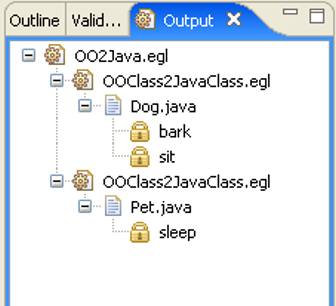
\includegraphics[scale=0.6]{images/TraceView}
  \end{center}
  \caption{Sample output from the traceability API.}
  \label{fig:traceability}
\end{figure}


\begin{lstlisting}[float=tbp, caption=Programmatically accessing the EGL traceability API (in Java)., label=lst:traceability, language=Java]
	IEolExecutableModule module = 
	  new EglTemplateFactoryModuleAdapter(new EglTemplateFactory());
	
	boolean parsed = module.parse(new File("myTemplate.egl"));
	
	if (parsed && module.getParseProblems().isEmpty()) {
		module.execute();

		Template base = module.getContext().getBaseTemplate();
		
		// traverse the template hierachy
		// display data 
		
	} else {
		// error handling
	}
\end{lstlisting}

\chapter{The Epsilon Comparison Language (ECL)}
\label{sec:ECL}

Model comparison is the task of identifying \emph{matching} elements between models. In general, \emph{matching} elements are elements that are involved in a relationship of interest. For example, before merging homogeneous models, it is essential to identify overlapping (common) elements so that they do not appear in duplicate in the merged model. Similarly, in heterogeneous model merging, it is a prerequisite to identify the elements on which the two models will be merged. Finally, in transformation testing, matching elements are pairs consisting of elements in the input model and their generated counterparts in the output model.

The aim of the Epsilon Comparison Language (ECL) is to enable users to specify comparison algorithms in a rule-based manner to identify pairs of matching elements between two models of potentially different metamodels and modelling technologies. In this section, the abstract and concrete syntax, as well as the execution semantics of the language, are discussed in detail.

%A comparison algorithm separates the model elements of the involved models into two categories: those that have matching elements in the opposite model and those that do not. Moreover, as the algorithm does not necessarily attempt to find matching elements for all the model elements of the involved models, the classification can be further refined to the following:
%
%\begin{enumerate}
%	\item Elements for which matching elements exist in the opposite model
%	\item Elements for which matching elements do not exist in the opposite model
%	\begin{enumerate}
%	\item Elements for which matching has been attempted but no matching elements has been found
%	\item Elements for which no matching has been attempted
%	\end{enumerate}
%\end{enumerate}

\section{Abstract Syntax}

In ECL, comparison specifications are organized in modules (\emph{EcLModule}). As illustrated in Figure \ref{fig:ECL}, EclModule extends EOLLibraryModule which means that it can contain user-defined operations and import other library modules and ECL modules. Apart from operations, an ECL module contains a set of match-rules (\emph{MatchRule}) and a set of \emph{pre} and \emph{post} blocks than run before and after all comparisons, respectively.

\emph{MatchRules} enable users to perform comparison of model elements at a high level of abstraction. Each match-rule declares a name, and two parameters (\emph{leftParameter} and \emph{rightParameter}) that specify the types of elements it can compare. It also optionally defines a number of rules it inherits (\emph{extends}) and if it is \emph{abstract}, \emph{lazy} and/or \emph{greedy}. The semantics of the latter are discussed shortly.

\begin{landscape}
\begin{figure}
	\centering
		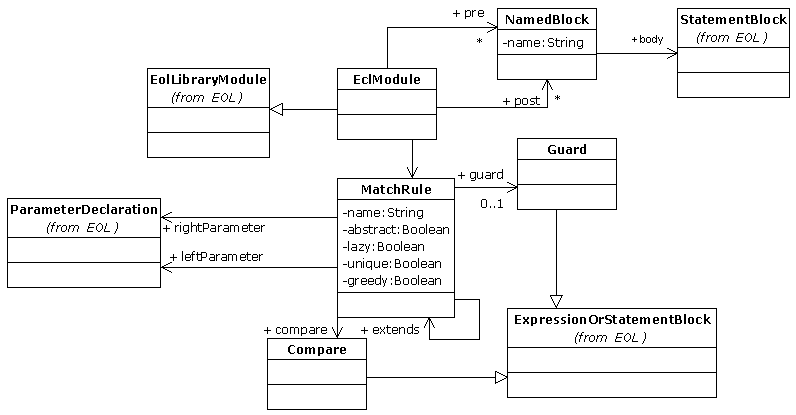
\includegraphics{images/EclAbstractSyntax.png}
	\caption{ECL Abstract Syntax}
	\label{fig:ECL}
\end{figure}
\end{landscape}

A match rule has three parts. The \emph{guard} part is an EOL expression or statement block that further limits the applicability of the rule to an even narrower range of elements than that specified by the \emph{left} and \emph{right} parameters. The \emph{compare} part is an EOL expression or statement block that is responsible for comparing a pair of elements and deciding if they match or not. Finally, the \emph{do} part is an EOL expression or block that is executed if the \emph{compare} part returns true to perform any additional actions required.

\emph{Pre} and \emph{post} blocks are named blocks of EOL statements which as discussed in the sequel are executed before and after the match-rules have been executed respectively.

\section{Concrete Syntax}

The concrete syntax of a match-rule is displayed in Listing \ref{lst:MatchRuleConcreteSyntax}.

\begin{lstlisting}[caption=Concrete Syntax of a MatchRule, label=lst:MatchRuleConcreteSyntax, language=ECL]

(@lazy)?
(@greedy)?
(@abstract)? 
rule <name> 
	match <leftParameterName>:<leftParameterType>
	with <rightParameterName>:<rightParameterType>
	(extends (<ruleName>,)*<ruleName>)? {
	
	(guard (:expression)|({statementBlock}))?
	
	compare (:expression)|({statementBlock})
	
	(do {statementBlock})?
	
}
\end{lstlisting}

\emph{Pre} and \emph{post} blocks have a simple syntax that, as presented in Listing \ref{lst:EclPrePostConcreteSyntax}, consists of the identifier (\emph{pre} or \emph{post}), an optional name and the set of statements to be executed enclosed in curly braces.

\begin{lstlisting}[caption=Concrete Syntax of Pre and Post blocks, label=lst:EclPrePostConcreteSyntax, language=ECL]
(pre|post) <name> {
	statement+
}
\end{lstlisting}

\section{Execution Semantics}

\subsection{Rule and Block Overriding}

An ECL module can import a number of other ECL modules. In such a case, the importing ECL module inherits all the rules and pre/post blocks specified in the modules it imports (recursively). If the module specifies a rule or a pre/post block with the same name, the local rule/block overrides the imported one respectively.

\subsection{Comparison Outcome}

As illustrated in Figure \ref{fig:ECLRuntime}, the result of comparing two models with ECL is a trace (\emph{MatchTrace}) that consists of a number of matches (\emph{Match}). Each match holds a reference to the objects from the two models that have been compared (\emph{left} and \emph{right}), a boolean value that indicates if they have been found to be \emph{matching} or not, a reference to the \emph{rule} that has made the decision, and a Map (\emph{info}) that is used to hold any additional information required by the user (accessible at runtime through the \emph{matchInfo} implicit variable). During the matching process, a second, temporary, match trace is also used to detect and resolve cyclic invocation of match-rules as discussed in the sequel.

\begin{figure}
	\centering
		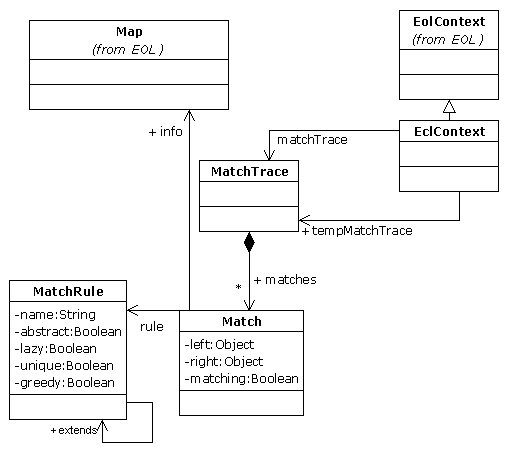
\includegraphics{images/ECLRuntime.png}
	\caption{ECL Match Trace}
	\label{fig:ECLRuntime}
\end{figure}

\subsection{Rule Execution Scheduling}

Non-abstract, non-lazy match-rules are evaluated automatically by the execution engine in a top-down fashion - with respect to their order of appearance - in two passes. In the first pass, each rule is evaluated for all the pairs of instances in the two models that have a type-of relationship with the types specified by the \emph{leftParameter} and \emph{rightParameter} of the rule. In the second pass, each rule that is marked as \emph{greedy} is executed for all pairs that have not been compared in the first pass, and which have a kind-of relationship with the types specified by the rule. In both passes, to evaluate the compare part of the rule, the guard must be satisfied.

Before the compare part of a rule is executed, the compare parts of all of the rules it extends (super-rules) must be executed (recursively). Before executing the compare part of a super-rule, the engine verifies that the super-rule is actually applicable to the elements under comparison by checking for type conformance and evaluating the guard part of the super-rule.

If the compare part of a rule evaluates to true, the optional do part is executed. In the do part the user can specify any actions that need to be performed for the identified matching elements, such as to populate the \emph{info} map of the established \emph{match} with additional information. Finally, a new match is added to the match trace that has its \emph{matching} property set to the logical conjunction of the results of the evaluation of the compare parts of the rule and its super-rules.

\subsection{The \emph{matches()} built-in operation}

To refrain from performing duplicate comparisons and to de-couple match-rules from each other, ECL provides the built-in \emph{matches(opposite : Any)} operation for model elements and collections. When the \emph{matches()} operation is invoked on a pair of objects, it queries the main and temporary match-traces to discover if the two elements have already been matched and if so it returns the cached result of the comparison. Otherwise, it attempts to find an appropriate match rule to compare the two elements and if such a rule is found, it returns the result of the comparison, otherwise it returns false. Unlike the top-level execution scheme, the \emph{matches()} operation invokes both \emph{lazy} and \emph{non-lazy} rules.

In addition to objects, the \emph{matches} operations can also be invoked to match pairs of collections of the same type (e.g. a Sequence against a Sequence). When invoked on ordered collections (i.e. \emph{Sequence} and \emph{OrderedSet}), it examines if the collections have the same size and each item of the source collection matches with the item of the same index in the target collection. Finally, when invoked on unordered collections (i.e. \emph{Bag} and \emph{Set}), it examines if for each item in the source collection, there is a matching item in the target collection irrespective of its index. Users can also override the built-in \emph{matches} operation using user-defined operations with the same name, as discussed in Section \ref{sec:Design.EOL.FeatureNavigation}, that loosen or strengthen the built-in semantics.

\subsection{Cyclic invocation of \emph{matches()}}

Providing the built-in \emph{matches} operation significantly simplifies comparison specifications. It also enhances decoupling between match-rules from each other as when a rule needs to compare two elements that are outside its scope, it does not need to know/specify which other rule can compare those elements explicitly.

On the other hand, it is possible - and quite common indeed - for two rules to implicitly invoke each other. For example consider the match rule of Listing \ref{lst:Tree2Tree} that attempts to match nodes of the simple Tree metamodel displayed in Figure \ref{fig:Tree}.

\begin{figure}
	\centering
		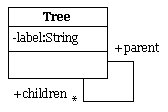
\includegraphics{images/metamodels/Tree.png}
	\caption{The Tree Metamodel}
	\label{fig:Tree}
\end{figure}

\begin{lstlisting}[caption=The Tree2Tree rule, label=lst:Tree2Tree, language=ECL]
rule Tree2Tree 
	match l : T1!Tree
	with r : T2!Tree {
	
	compare : l.label = r.label and 
		l.parent.matches(r.parent) and
		l.children.matches(r.children)
}
\end{lstlisting}

The rule specifies that for two Tree nodes (\emph{l} and \emph{r}) to match, they should have the same label, belong to matching parents and have matching children. In the absence of a dedicated mechanism for cycle detection and resolution, the rule would end up in an infinite loop. To address this problem, ECL provides a temporary match-trace which is used to detect and resolve cyclic invocations of the \emph{match()} built-in operation.

As discussed above, a match is added to the primary match-trace as soon as the compare part of the rule has been executed to completion. By contrast, a temporary match (with its \emph{matching} property set to \emph{true}) is added to the temporary trace before the compare part is executed. In this way, any subsequent attempts to match the two elements from invoked rules will not re-invoke the rule. Finally, when a top-level rule returns, the temporary match trace is reset.

\section{Fuzzy and Dictionary-based String Matching}
\label{sec:FuzzyComparison}

In the example of Listing \ref{lst:Tree2Tree}, the rule specifies that to match, two trees must - among other criteria - have the same label. However, there are cases when a less-strict approach to matching string properties of model elements is desired. For instance, when comparing two UML models originating from different organizations, it is common to encounter ontologically equivalent classes which however have different names (e.g. Client and Customer). In this case, to achieve a more sound matching, the use of a dictionary or a lexical database (e.g. WordNet \cite{Wordnet}) is necessary. Alternatively, fuzzy string matching algorithms such as those presented in \cite{FuzzyStringMatching} can be used.

As several such tools and algorithms have been implemented in various programming languages, it is a sensible approach to reuse them instead of re-implementing them. For example, in Listing \ref{lst:FuzzyTree2Tree} a wrapper for the Simmetrics \cite{Simmetrics} fuzzy string comparison tool is used to compare the labels of the trees using the Levenshtein \cite{Levenshtein} algorithm. To achieve this, line 11 invokes the \emph{fuzzyMatch()} operation defined in lines 16-18 which uses the simmterics native tool (instantiated in lines 2-4) to match the two labels using their Levenshtein distance with a threshold of 0.5.

\begin{lstlisting}[caption=The FuzzyTree2Tree rule, label=lst:FuzzyTree2Tree, language=ECL]
pre {
	var simmetrics = 
		new Native("org.epsilon.ecl.tools.
			textcomparison.simmetrics.SimMetricsTool"); 
}

rule FuzzyTree2Tree 
	match l : T1!Tree
	with r : T2!Tree {
	
	compare : l.label.fuzzyMatch(r.label) and 
		l.parent.matches(r.parent) and
		l.children.matches(r.children)
}

operation String fuzzyMatch(other : String) : Boolean {
	return simmetrics.similarity(self,other,"Levenshtein") > 0.5;
}\end{lstlisting}

\section{Interactive Matching}
\label{sec:InteractiveModelComparison}

Using the user interaction features discussed in Section \ref{sec:Design.EOL.UserInput} the comparison can become interactive by replacing the \emph{fuzzyMatch} operation of listing \ref{lst:FuzzyTree2Tree} with the one specified in Listing \ref{lst:InteractiveTree2TreeComparison}. The fuzzyMatch operation of Listing \ref{lst:InteractiveTree2TreeComparison}, performs the fuzzy string comparison and -- as the previous version -- if the result is greater than 0.5 it returns true. However, in this updated version if the result is lower than 0.5 but greater than 0.3, it prompts the user to confirm if the two strings match, and if it is lower than 0.3 it returns false.

\begin{lstlisting}[caption=An interactive version of the fuzzyMatch operation of Listing \ref{lst:FuzzyTree2Tree}, label=lst:InteractiveTree2TreeComparison, language=ECL]
operation String fuzzyMatch(other : String) : Boolean {
	var similarity : Real;
	similarity = simmetrics.similarity(self,other,"Levenshtein");
	if (similarity > 0.5) {
		return true;
	}
	else if (similarity > 0.3) {
		return UserInput.confirm(self + " matches " + other + "?");
	}
	else {
		return false;
	}
}\end{lstlisting}

\section{Exploiting the Comparison Outcome}

Users can query and modify the match trace calculated during the comparison process in the post sections of the module or export it into another application or Epsilon program. For example, in a post section, the trace can be printed to the default output stream or serialized into a model of an arbitrary metamodel. In another use case, the trace may be exported to be used in the context of a validation module that will use the identified matches to evaluate inter-model constraints, or in a merging module that will use the matches to identify the elements on which the two models will be merged. The topic of interoperability - that includes importing and exporting objects - between modules expressed in different Epsilon languages is discussed in Chapter \ref{chp:Workflow}.

\chapter{The Epsilon Merging Language (EML)}
\label{sec:EML}

The aim of EML is to contribute model merging capabilities to Epsilon. More specifically, EML can be used to merge an arbitrary number of input models of potentially diverse metamodels and modelling technologies. This section provides a discussion on the motivation for implementing EML, its abstract and concrete syntax, as well as its execution semantics. It also provides two examples of merging homogeneous and heterogeneous models.

\section{Motivation}

A mechanism that enables automatically merging models on a set of established correspondences has a number of applications in a model driven engineering process. For instance, it can be used to unify two complementary, but potentially overlapping, models that describe different views of the same system. In another scenario, it can be used to merge a core model with an aspect model (potentially conforming to different metamodels), as discussed in \cite{MDAGuide} where a core \emph{Platform Independent Model (PIM)} is merged with a \emph{Platform Definition Model (PDM)}, that contributes platform-specific aspects, into a \emph{Platform Specific Model (PSM)}.

\subsection{Phases of Model Merging}

Existing research \cite{Pottinger2003,Batini1986} has demonstrated that model merging can be decomposed into four distinct phases: comparison, conformance checking, merging and reconciliation (or restructuring).

\paragraph{Comparison Phase} In the comparison phase, correspondences between equivalent elements of the source models are identified, so that such elements are not propagated in duplicate in the merged model.

%In \cite{ModelWeaver} the ModelWeaver, a generic framework for capturing different types of relationships, such as match relationships, between elements of different models is illustrated.  Matching pairs of elements can be defined graphically through a tree-based user interface and declared relationships can be stored in a separate \textit{weaving model}. Weaving models can be used later by other tools such as model transformation or model merging tools. While this is a flexible approach that promotes reuse, it does not scale well since manual definition of each matching pair is a labour intensive process.

%In \cite{Alanen2003}, matching is performed using persistent model-element identifiers (i.e. using the $xmi.id$ identifier). However, this only applies to comparison of models that are versions of a common ancestor. In \cite{Gray2005}, matching is performed by comparing the \textit{names} of the elements of the two models. Nevertheless, there are model elements that do not have a name (e.g. instances of the $Multiplicity$ UML metaclass) to compare.

\paragraph{Conformance Checking Phase} In this phase, elements that have been identified as matching in the previous phase are examined for conformance with each other. The purpose of this phase is to identify potential conflicts that would render merging infeasible. The majority of proposed approaches, such as \cite{Letkeman2005}, address conformance checking of models complying with the same metamodel. 
 
\paragraph{Merging Phase}
Several approaches have been proposed for the merging phase. In \cite{Pottinger2003,Melnik2003}, graph-based algorithms for merging models of the same metamodel are proposed. In \cite{Letkeman2005}, an interactive process for merging of UML 2.0 models is presented. There are at least two weaknesses in the methods proposed so far. First, they only address the issue of merging models of the same metamodel, and some of them address a specific metamodel indeed. Second, they use an inflexible merging algorithm and do not provide means for extending or customizing its logic.

\paragraph{Reconciliation and Restructuring Phase}
After the merging phase, the target model may contain inconsistencies that need fixing. In the final step of the process, such inconsistencies are removed and the model is \textit{polished} to acquire its final form. Although the need for a reconciliation phase is discussed in \cite{Batini1986,Melnik2003}, in the related literature the subject is not explicitly targeted.

\subsection{Relationship between Model Merging and Model Transformation}

A merging operation is a transformation in a general sense, since it transforms some input (source models) into some output (target models). However, as discussed throughout this section, a model merging facility has special requirements (support for comparison, conformance checking and merging pairs of input elements) that are not required for typical \textit{one-to-one} or \textit{one-to-many} transformations \cite{Czarnecki2003} and are therefore not supported by contemporary model transformation languages.

\section{Realizing a Model Merging Process with Epsilon}

The first two steps of the process described above can be realized with existing languages provided by Epsilon. As discussed in Section \ref{sec:ECL}, the comparison step can be realized with the Epsilon Comparison Language (ECL). Following that, the Epsilon Validation Language (EVL) can be used to validate the identified correspondences using the match trace calculated by ECL. The Epsilon Merging Language (EML) presented below provides support for the last two steps of the process (merging and reconciliation/restructuring).

\section{Abstract Syntax}

In EML, merging specifications are organized in modules (\emph{EmlModule}). As displayed in Figure \ref{fig:EmlAbstractSyntax}, \emph{EmlModule} inherits from \emph{EtlModule}.

\begin{sidewaysfigure}
  \centering
  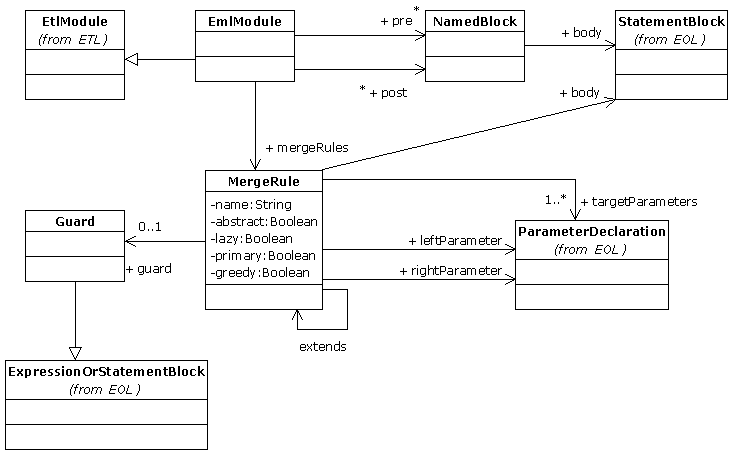
\includegraphics{images/EmlAbstractSyntax.png}
  \caption{The Abstract Syntax of EML}
  \label{fig:EmlAbstractSyntax}
\end{sidewaysfigure}

By extending \emph{EtlModule}, an EML module can contain a number of transformation rules and user-defined operations. An EML module can also contain one or more merge rules as well as a set of \emph{pre} and \emph{post} named EOL statement blocks. As usual, \emph{pre} and \emph{post} blocks will be run before and after all rules, respectively.

Each merge rule defines a name, a left, a right, and one or more target parameters. It can also extend one or more other merge rules and be defined as having one or more of the following properties: abstract, greedy, lazy and primary.

\section{Concrete Syntax}

Listing \ref{lst:EmlConcreteSyntax} demonstrates the concrete syntax of EML merge-rules.

\begin{lstlisting}[float=tbp, caption=Concrete syntax of an EML merge-rule, label=lst:EmlConcreteSyntax, language=EML]
(@abstract)?
(@lazy)?
(@primary)?
(@greedy)?
rule <name>
	merge <leftParameter>
	with <rightParameter>
	into (<targetParameter>(, <targetParameter>)*)?
	(extends <ruleName>(, <ruleName>)*)? {

	statementBlock
	
}
\end{lstlisting}

\emph{Pre} and \emph{post} blocks have a simple syntax that, as presented in Listing \ref{lst:EmlPrePostConcreteSyntax}, consists of the identifier (\emph{pre} or \emph{post}), an optional name and the set of statements to be executed enclosed in curly braces.

\begin{lstlisting}[float=tbp, caption=Concrete Syntax of Pre and Post blocks, label=lst:EmlPrePostConcreteSyntax, language=EML]
(pre|post) <name> {
	statement+
}
\end{lstlisting}

\section{Execution Semantics}

\subsection{Rule and Block Overriding}
An EML module can import a number of other EML and ETL modules. In this case, the importing EML module inherits all the rules and pre/post blocks specified in the modules it imports (recursively). If the module specifies a rule or a pre/post block with the same name, the local rule/block overrides the imported one respectively.

\subsection{Rule Scheduling}
When an EML module is executed, the \emph{pre} blocks are executed in the order in which they have been defined.

Following that, for each \emph{match} of the established \emph{matchTrace} the applicable non-abstract, non-lazy merge rules are executed. When all \emph{matches} have been merged, the transformation rules of the module are executed on all applicable elements - that have not been merged - in the models.

Finally, after all rules have been applied, the \emph{post} blocks of the module are executed.

\subsection{Rule Applicability}
By default, for a merge-rule to apply to a \emph{match}, the \emph{left} and \emph{right} elements of the match must have a \emph{type-of} relationship with the \emph{leftParameter} and \emph{rightParameter} of the rule respectively. This can be relaxed to a \emph{kind-of} relationship by specifying that the merge rule is \emph{greedy} (using the \emph{@greedy} annotation in terms of concrete syntax).

\subsection{Source Elements Resolution}

As with model transformation, in model merging it is often required to resolve the counterparts of an element of a source model into the target models. In EML, this is achieved by overloading the semantics of the \emph{equivalents()} and \emph{equivalent()} operations defined by ETL. In EML, in addition to inspecting the transformation trace and invoking any applicable transformation rules, the \emph{equivalents()} operation also examines the \emph{mergeTrace} (displayed in Figure \ref{fig:EmlRuntime}) that stores the results of the application of merge-rules and invokes any applicable (both lazy and non-lazy) rules.

Similarly to ETL, the order of the results of the \emph{equivalents()} operation respects the order of the (merge or transform) rules that have produced them. An exception to that occurs if one of the rules has been declared as primary, in which case its results are prepended to the list of elements returned by equivalent.

\begin{figure}
	\centering
		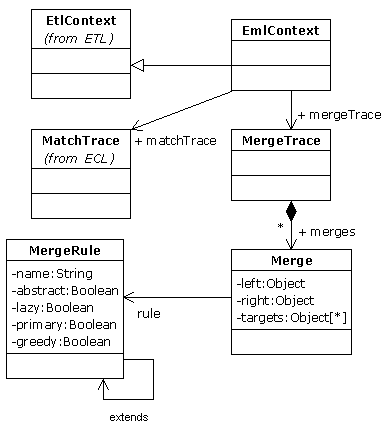
\includegraphics{images/EmlRuntime.png}
	\caption{The EML runtime}
	\label{fig:EmlRuntime}
\end{figure}

\section{Homogeneous Model Merging Example}

In this scenario, two models conforming to the Graph metamodel need to be merged. The first step is to compare the two graphs using the ECL module of Listing \ref{lst:CompareGraph}.

\begin{lstlisting}[float=tbp, caption=ECL module for comparing two instances of the Graph metamodel, label=lst:CompareGraph, language=ECL, tabsize=2]
rule MatchNodes /*@\label{line:MatchNodes}@*/
	match l : Left!Node
	with r : Right!Node {

	compare : l.label = r.label
}

rule MatchEdges /*@\label{line:MatchEdges}@*/
	match l : Left!Edge
	with r : Right!Edge {

	compare : l.source.matches(r.source)
		and l.target.matches(r.target)
}

rule MatchGraphs /*@\label{line:MatchGraphs}@*/
	match l : Left!Graph
	with r : Right!Graph {

	compare : true
}
\end{lstlisting}

The \emph{MatchNodes} rule in line \ref{line:MatchNodes} defines that two nodes match if they have the same label. The \emph{MatchEdges} rule in line \ref{line:MatchEdges} specifies that two edges match if both their source and target nodes match (regardless of whether the labels of the edges match or not as it is assumed that there can not be two distinct edges between the same nodes). Finally, since only one instance of Graph is expected to be in each model, the \emph{MatchGraphs} rule in line \ref{line:MatchGraphs} returns \emph{true} for any pair of Graphs\footnote{Both assumptions can be checked using EVL before matching/merging takes place but this is out of the scope of this example}.

Having established the necessary correspondences between matching elements of the two models, the EML specification of listing \ref{lst:MergeGraphs}.

\begin{lstlisting}[float=tbp, label=lst:MergeGraphs, caption=EML module for merging two instances of the Graph metamodel on the correspondences identified in Listing \ref{lst:CompareGraph} , language=EML]
import "Graphs.etl";

rule MergeGraphs /*@\label{line:MergeGraphs}@*/
	merge l : Left!Graph
	with r : Right!Graph
	into t : Target!Graph {
	
	t.label = l.label + " and " + r.label;
	
}

@abstract
rule MergeGraphElements /*@\label{line:MergeGraphElements}@*/
	merge l : Left!GraphElement
	with r : Right!GraphElement
	into t : Target!GraphElement {
	
	t.graph ::= l.graph;
	
}

rule MergeNodes /*@\label{line:MergeNodes}@*/
	merge l : Left!Node
	with r : Right!Node
	into t : Target!Node 
	extends GraphElements {
	
	t.label = "c_" + l.label;
	
}
rule MergeEdges /*@\label{line:MergeEdges}@*/
	merge l : Left!Edge
	with r : Right!Edge
	into t : Target!Edge 
	extends GraphElements {
	
	t.source ::= l.source;
	t.target ::= l.target;
	
}
\end{lstlisting}

In line \ref{line:MergeGraphs}, the \emph{MergeGraphs} merge rule specifies that two matching Graphs (\emph{l} and \emph{r}) are to be merged into one Graph \emph{t} in the target model that has as a label, the concatenation of the labels of the two input graphs separated using 'and'. The \emph{mergeNodes} rule In line \ref{line:MergeNodes} specifies that two matching Nodes are merged into a single Node in the target model. The label of the merged node is derived by concatenating the c (for common) static string with the label of the source Node from the left model. Similarly, the \emph{MergeEdges} rule specifies that two matching Edges are merged into a single Edge in the target model. The source and target nodes of the merged Edge are set to the equivalents (::=) of the source and target nodes of the edge from the left model.

To reduce duplication, the \emph{MergeNodes} and \emph{MergeEdges} rules extend the abstract \emph{MergeGraphElements} rule specified in line \ref{line:MergeGraphElements} which assigns the \emph{graph} property of the graph element to the equivalent of the left graph.

The rules displayed in Listing \ref{lst:MergeGraphs} address only the matching elements of the two models. To also copy the elements for which no equivalent has been found in the opposite model, the EML module imports the ETL module of Listing \ref{lst:CopyGraph}.

\begin{lstlisting}[float=tbp, caption=The Graphs.etl ETL transformation module, label=lst:CopyGraph, language=ETL]
rule TransformGraph 
	transform s : Source!Graph
	to t : Target!Graph {
	
	t.label = s.label;
	
}

@abstract
rule TransformGraphElement 
	transform s : Source!GraphElement
	to t : Target!GraphElement {
	
	t.graph ::= s.graph;
}

rule TransformNode /*@\label{line:TransformNode}@*/
	transform s : Source!Node
	to t : Target!Node 
	extends TransformGraphElement {
	
	t.label = s.graph.label + "_" + s.label;
}

rule TransformEdge 
	transform s : Source!Edge
	to t : Target!Edge 
	extends TransformGraphElement {
	
	t.source ::= s.source;
	t.target ::= s.target;	
} 
\end{lstlisting}

The rules of the ETL module apply to model elements of both the Left and the Right model as both have been aliased as Source. Of special interest is the TransformNode rule in line \ref{line:TransformNode} that specifies that non-matching nodes in the two input models will be transformed into nodes in the target model the labels of which will be a concatenation of their input graph and the label of their counterparts in the input models.

Executing the ECL and EML modules of Listings \ref{lst:CompareGraph} and \ref{lst:MergeGraphs} on the exemplar models displayed in Figures \ref{fig:LeftGraph} and \ref{fig:RightGraph} creates the target model of Figure \ref{fig:TargetGraph}.

\begin{figure}
	\centering
		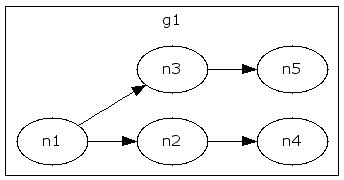
\includegraphics{images/LeftGraph.png}
	\caption{Left input model}
	\label{fig:LeftGraph}
\end{figure}


\begin{figure}
	\centering
		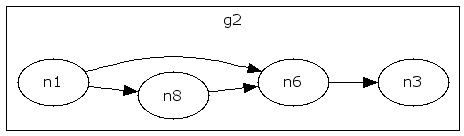
\includegraphics{images/RightGraph.png}
	\caption{Right input model}
	\label{fig:RightGraph}
\end{figure}


\begin{figure}
	\centering
		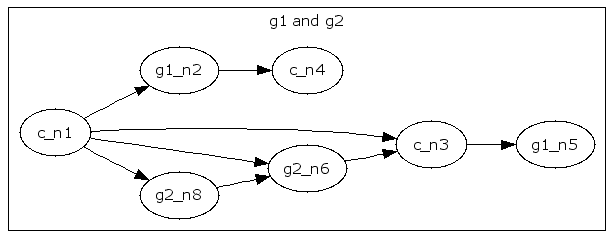
\includegraphics{images/MergedGraph.png}
	\caption{Target model derived by merging the models of Figures \ref{fig:LeftGraph} and \ref{fig:RightGraph}}
	\label{fig:TargetGraph}
\end{figure}

\chapter{Implementing a New Task-Specific Language}
\label{sec:Design.ImplementingANewLanguage}

Although Epsilon already provides languages for a wide range of model management tasks, additional tasks that could benefit from the convenience syntax and dedicated semantics of a task-specific language are likely to be identified in the future. Thus, this section distils the experiences obtained through the construction of existing task-specific languages to provide guidance on how to identify a task for which a dedicated language can be beneficial and develop the respective task-specific language for it atop the infrastructure provided by Epsilon.

\section{Identifying the need for a new language}

The first step of the process of constructing a new task-specific language is to identify a specific task for which a dedicated language is more appropriate than the general-purpose EOL. Typically, recurring syntactic and semantic patterns that emerge when attempting to implement the task using EOL indicate that a new task-specific language may be useful.

For example, before the introduction of the Epsilon Comparison Language, pure EOL was being used to perform model comparison. A simple comparison specification that establishes name-based matches between classes/attributes and tables/columns between two OO and DB models respectively using EOL is demonstrated in Listing \ref{lst:ComparisonEOL}.

Two patterns can be readily detected by inspecting the EOL code in Listing \ref{lst:ComparisonEOL}. First, explicit variables (\emph{matchingCT}, \emph{matchingAT}) are defined to capture the matching elements (class-table and attribute-column)identified during the comparison process. Also, to check all elements of one type (classes against tables and attributes against columns) repeated for statements are used in lines \ref{line:For11}--\ref{line:For12} and \ref{line:For21}--\ref{line:For22}. By contrast, Listing \ref{lst:ComparisonECL} which is specified using the task-specific ECL language does not include such low-level information. Instead it defines only the types of elements that need to be compared and the criteria on which comparison must performed and leaves the mundane tasks of scheduling and maintaining the match trace to the execution engine.

\begin{lstlisting}[basicstyle=\ttfamily\footnotesize, flexiblecolumns=true, numbers=left, nolol=true, caption=Comparing an OO model with a DB model using EOL, label=lst:ComparisonEOL, language=EOL, tabsize=2]
var matchingCT : Sequence; /*@\label{line:MatchTrace1}@*/
var matchingAC : Sequence; /*@\label{line:MatchTrace2}@*/
for (c in OO!Class.allInstances) { /*@\label{line:For11}@*/
	for (t in DB!Table.allInstances) { /*@\label{line:For12}@*/
		if (t.name = c.name) {
			matchingCT.add(Sequence{c,t});
			for (att in c.attributes) { /*@\label{line:For21}@*/
				for (col in t.columns) { /*@\label{line:For22}@*/
					if (att.name = c.name) {
						matchingAC.add(Sequence{att, col});
					}
				}
			}
		}
	}
}
\end{lstlisting}

\begin{lstlisting}[basicstyle=\ttfamily\footnotesize, flexiblecolumns=true, numbers=left, nolol=true, caption=Comparing an OO model with a DB model using ECL, label=lst:ComparisonECL, language=ECL, tabsize=2]
rule ClassTable
	match c : OO!Class
	with t : DB!Table {
	
	compare : c.name = t.name
}

rule AttributeColumn
	match a : OO!Attribute 
	with c : DB!Column {
	
	compare : a.name = c.name and
		a.class.matches(c.table)
}
\end{lstlisting}

\section{Eliciting higher-level constructs from recurring patterns}

Once recurring patterns, such as those discussed above, have been identified, the next step of the process is to derive higher level constructs from them. For instance, in the previous example, the nested for loops and the explicit trace variable declaration and population have been replaced by task-specific match rules.

Introducing higher-level involves defining its abstract and concrete syntax as well as its connection points with the underlying infrastructure. For example, in the case of ECL, the types of match rules are EOL model element types, the \emph{guard} and \emph{check} parts of a rule are EOL expressions or statements blocks and the \emph{pre} and \emph{post} blocks as well as the \emph{do} part of each rule are blocks of EOL statements.

\section{Implement Execution Semantics and Scheduling}

Once higher-level constructs (e.g. task-specific rules) have been identified and specified, their execution semantics and scheduling must be implemented similarly to what has been done for existing languages. Development of existing languages has demonstrated that task-specific constructs often need to provide more than one modes of execution (e.g. the \emph{lazy} and \emph{greedy} modes of ETL transformation rules discussed in Section \ref{sec:ETL.ExecutionSemantics}). 

A lightweight way to easily provide new execution modes and semantics for rules and user-defined operations without modifying the syntax of the language and introducing new keywords that may conflict with existing code, is through the annotations mechanism provided by EOL (see Section \ref{sec:Design.EOL.Annotations}). This approach has been adopted for the definition a small unit-testing language (EUnit), which is discussed in detail in \cite{EUnit}.

\section{Overriding Semantics}

In certain cases, it is useful to modify the semantics of certain constructs in EOL to meet the purposes of the task-specific language. An example of such a modification occurs in EVL where -- as discussed in Section \ref{sec:Design.EVL.ExecutionSemantics} -- the scope of the variables defined in \emph{guard} expression/block is extended so that variables can be reused in the context of non-nested blocks such as the \emph{title}, and \emph{check} parts of the invariant. Another example of overriding the semantics of EOL is the implementation of the special assignment operator ($::=$) by ETL which was discussed in \ref{sec:Design.ETL.SpecialAssignmentOperator}.




